\chapter{Estimation of variance components and effective degrees of freedom in two-phase proteomic experiments}

\section{Introduction}
\label{sec:introChap5}
In Chapter 2, we described the methodology needed to construct theoretical ANOVA tables for two-phase experiments. Chapters 3 and 4 then developed methods for constructing and searching for optimal designs for Phase 2 proteomics experiments when the Phase 1 experiment is arranged in a completely randomised design (CRD), a randomised complete block design (RCBD), or a balanced incomplete block design (BIBD). Theoretical ANOVA tables were shown to be a very useful tool for investigating and comparing the properties of optimal designs of different Phase 2 experiments for a given Phase 1 design. This chapter presents a third component of this thesis in estimating variance components (VCs) based on expected mean squares (EMS) of the theoretical ANOVA table, where we focus on the Residual mean squares (MS) of the same stratum for testing the Treatment effects. The example of this chapter is in the Between Animals Within Runs stratum. In addition, the Phase 2 Block (Run) effects are assumed to be random may allow us to obtain a test that effectively has higher degrees of freedom (DF) for the Residual MS, namely the \emph{effective degrees of freedom} (EDF).  

%Consider where a Phase 1 experiment is arranged in a CRD with $s_b = 3$ biological replicates of each of $\nu = 2$ treatments, meaning the total number of animals is 6. If a four-plex system is used, the animals cannot be allocated to runs such that animals effects are orthogonal to run effects. Hence, some animal information is contained in the Between Runs stratum. This chapter aims to show how to recover some of this animal information from the Between Runs stratum, which resulting in higher residual degrees of freedom (DF) for estimating the variances of the treatment effects. This adjusted DF is known as the \emph{effective degrees of freedom} (EDF). 

\cite{Jarrett2008} demonstrated that given the same design at Phase 1, the choice of design at Phase 2 can affect the analysis of a micro-array experiment. MudPIT-iTRAQ$^{\rm TM}$ experiments have their own unique set of problems. Either a four-plex or eight-plex labelling system can be used for the Phase 2 proteomics experiment, which allows researchers to measure either four or eight biological samples simultaneously. The EDF provide us with another property by which we can compare designs using four- and eight-plex systems, which we will apply to some of the optimal designs of the Phase 2 experiments found in Chapters 3 and 4.

%The EDF are computed based on the estimated variance components (VCs). Two methods of estimating VCs are discussed in this chapter. The first method uses a linear combination (LC) of the residual expected mean squares (EMS) from the theoretical ANOVA table. The second method attempts to improve the estimation of VCs using restricted maximum likelihood (REML) \citep{Patterson1971}. The EDF are then computed from the first two moments of an approximate $\chi^2$ distribution using the Satterthwaite approximation \citep{Satterthwaite1946}.
  
This Chapter first uses an optimal design, described in Section~\ref{sec:expDes}, to illustrate the estimation of VCs in Section~\ref{sec:estVC}. Based on the VCs estimates, the approximation method for the EDF is then shown in Section~\ref{sec:estEDF}. Section~\ref{sec:expCRD} compares the EDF between the Phase 2 design with four-plex and eight-plex systems given the same Phase 1 experiment arranged in a CRD. Section~\ref{sec:expRCBD} compares the EDF between four Phase 2 designs, given the same Phase 1 experiment is arranged in a RCBD, using two different confounding schemes when the Phase 1 Block effects are intentionally confounded with Tag effects or Phase 1 Block effects are intentionally confounded with Run effects, and between the four-plex and eight-plex systems.   

\section{An illustrative example}
\label{sec:expDes}
This section presents the most trivial example of a two-phase experiment, in which the Phase 1 experiment is arranged in a CRD with $\nu = 2$ treatments assigned to $n_a = 6$ animals. The layout of the Phase 1 design consists of Treatment \textit{a} assigned to Animals \textit{A}, \textit{C} and \textit{E}, and Treatment \textit{b} assigned to Animals \textit{B}, \textit{D} and \textit{F}. The samples from each animal are further split into $n_s$ sub-samples which are differentially labelled by $n_\gamma$ tags and analysed in $n_r$ runs of the Phase 2 experiment. The linear model of this Phase 2 experiment has been previously described in (\ref{eq:model}). 

\begin{table}[ht]
\centering
\itshape
\caption{Optimal design of Phase 2 proteomics experiment showing allocation of sub-samples from animals and treatment to runs and tags, when the Phase~1 experiment consists of $\nu = 2$ treatments assigned to each of $n_a = 6$ animals, $n_s = 2$ sub-samples are then taken from each animal, and labelled by $n_\gamma = 4$ tags and analysed in $n_r = 3$ runs of the Phase 2 MudPIT-iTRAQ$^{\rm TM}$ experiment.}
\begin{tabular}{c|cc:cc}
 & \multicolumn{4}{c}{{\bf Tag}} \\
{\bf Run}  & \textnormal{114} & \textnormal{115} & \textnormal{116} & \textnormal{117} \\ 
\hline 
\textnormal{1} & Db & Ca & Fb & Ea \\  
\textnormal{2} & Ca & Db & Ea & Fb \\  \hdashline
\textnormal{3} & Bb & Bb & Aa & Aa \\ 
\end{tabular} 
\label{tab:aniDes1Chap5}
\end{table}

An optimal design found using the methods described in Chapter 3 is shown in Table~\ref{tab:aniDes1Chap5}. There are several characteristics of this design: Runs 1 and 2 contain sub-samples from Animals $C$, $D$, $E$ and $F$, while Run 3 contains sub-samples from Animals $A$ and $B$. Thus, 1 of 4 DF associated with the Animal effects is confounded with 1 DF of the Between Runs stratum. Furthermore, Animals $B$, $C$ and $D$ are assigned to Tags 114 and 115, and Animals $A$, $E$ and $F$ are assigned to Tags 116 and 117. Thus, 1 DF associated with Tag effects is in the Between Animals stratum. Treatment effects are orthogonal to Run effects, as each run contains two of each treatment. There are unequal numbers of sub-samples from Treatment \textit{a} and \textit{b} labelled with each Tag resulting in some confounding between Treatment and Tag effects.

\begin{table}[ht]
\centering
\caption{Theoretical ANOVA table of the Phase 2 experiment in Table~\ref{tab:aniDes1Chap5}.}
\begin{tabular}{lrllll} 
\toprule 
\multicolumn{1}{l}{\textbf{Source of Variation}} & \multicolumn{1}{l}{\textbf{DF}}& \multicolumn{1}{l}{\textbf{MS}} & \multicolumn{1}{l}{\textbf{EMS}}& \multicolumn{1}{l}{$\bm{E_{\gamma}}$}&\multicolumn{1}{l}{$\bm{E_{\tau}}$}\\ 
\midrule 
Between Runs & & &  & & \\ 
\quad Between Animals & $1$ &$s_1^2$ & $ \sigma^2+2\sigma_{a}^2+4\sigma_{r}^2$ & & \\ 
\quad Within Animals & $1$ &$s_2^2$& $\sigma^2+4\sigma_{r}^2$ & & \\ \hline 
Within Runs &  &&  & & \\ 
\quad Between Animals &&  &  & & \\ 
\quad \quad Tag & $1$ && $\sigma^2+2\sigma_{a}^2+3\theta_{\gamma}+0.67\theta_{\tau}$ &$1$ & $0.111$\\ 
\quad \quad Treatment & $1$ & & $\sigma^2+2\sigma_{a}^2+5.33\theta_{\tau}$ & & $0.889$\\ 
\quad \quad Residual & $2$ &$s_3^2$& $\sigma^2+2\sigma_{a}^2$ & & \\ \hline 
\quad Within Animals &  &&  & & \\ 
\quad \quad Tag & $2$ && $\sigma^2+3\theta_{\gamma}$ &$1$ & \\ 
\quad \quad Residual & $3$ &$s_4^2$& $\sigma^2$ & & \\ 
\bottomrule 
\end{tabular} 
\label{tab:Phase2ANOVAChap5} 
\end{table} 

The theoretical ANOVA of the optimal design of the Phase 2 experiment in Table~\ref{tab:aniDes1Chap5} is presented in Table~\ref{tab:Phase2ANOVAChap5}. Notice that an additional column is present in this table, namely the mean square (MS) column, i.e.\ the estimated value of its corresponding EMS being computed from experimental data. There are four MS of interest, which contain only the random error variances: the Between Animals Between Runs MS ($s_1^2$), the Within Animals Between Runs MS ($s_2^2$), the Residual MS of the Between Animals Within Runs stratum ($s_3^2$) and the Residual MS of the Within Animals Within Runs stratum ($s_4^2$). These MS, also known as residual variances, are related to their associated EMS as follows 
\begin{eqnarray}
\label{eq:s1} s_1^2 &=&  \hat{\sigma}^2+2\hat{\sigma}_{a}^2+4\hat{\sigma}_{r}^2,\\
\label{eq:s2} s_2^2 &=&  \hat{\sigma}^2+4\hat{\sigma}_{r}^2,\\
\label{eq:s3} s_3^2 &=&  \hat{\sigma}^2+2\hat{\sigma}_{a}^2,\\
\label{eq:s4} s_4^2 &=&  \hat{\sigma}^2,
\end{eqnarray}
where $\hat{\sigma}^2$, $\hat{\sigma}_{a}^2$, and $\hat{\sigma}_{r}^2$ are the estimated between sub-samples, between animals, and between runs VCs, respectively. The $\hat{\sigma}^2$ is the residual variance from the Within Animals Within Runs stratum as shown in (\ref{eq:s4}). Subtracting (\ref{eq:s4}) from (\ref{eq:s3}) gives $\hat{\sigma}_{a}^2 = (s_3^2 - s_4^2)/2$. We then subtract (\ref{eq:s4}) from (\ref{eq:s2}) to solve for $\hat{\sigma}_{r}^2$, which gives $\hat{\sigma}_{r}^2 = (s_2^2 - s_4^2)/4.$ Following \cite{Jarrett2008}, this method of solving a system of linear equations to obtain estimates of the variance components is, from this point forward, referred to as the linear combination (LC) method. 

A purpose of constructing the theoretical ANOVA table is that it enables us to determine variances of Treatment effects, and therefore, a valid F-test for the Treatment effects can be obtained. The estimated Treatment difference between Treatments $a$ and $b$ is given by $(\bar{y}_{...}^{a..} - \bar{y}_{...}^{b..})$, which, for the Phase 2 design presented in Table~\ref{tab:aniDes1Chap5}, has variance 
\begin{equation}\label{eq:varTrt}
\operatorname{Var}(\bar{y}_{...}^{a..} - \bar{y}_{...}^{b..}) = \dfrac{\sigma^2+2\sigma_{a}^2}{3},
\end{equation}
where $\bar{y}_{...}^{i..}$ denotes the mean of the log-protein abundance values over all observations of Treatment $i$. The denominator of (\ref{eq:varTrt}) is 3, because each treatment group is replicated six times (with two sub-samples from each of three animals). The numerator of (\ref{eq:varTrt}), i.e.\ $\sigma^2+2\sigma_{a}^2$, can be estimated directly from the residual variance in the Within Animals Within Runs stratum, the same stratum in which the Treatment effects are being estimated. 

If Run effects are regarded as fixed effects, the row of Table~\ref{tab:Phase2ANOVAChap5} containing $\sigma_r^2$ is not available to be used, i.e.\ $s_1^2$ and $s_2^2$, which implies that the estimate of variance of the Treatment effects will be based solely on $s_3^2$ with 2 DF. If the Run effects are assumed to be random effects, we can recover extra information about $\sigma_a^2$ from $s_1^2$, defined in (\ref{eq:s1}), as well as information about $\sigma^2$ in the other residual variances. Thus, we can then improve the estimate of $\hat{\sigma}^2+2\hat{\sigma}_{a}^2$ either via the LC method as illustrated above, or by using restricted maximum likelihood (REML) approach to estimate the VC. How this may be achieved is discussed in Section~\ref{sec:estVC}.

\section{Estimation of variance components}
\label{sec:estVC}
The theoretical ANOVA in Table~\ref{tab:Phase2ANOVAChap5} identified four MS, with expected values $\xi_i^2$ and $\upsilon_i$ DF ($i = 1,\dots,4$), which are available for estimation of the VCs defined by $\bm{\varsigma} = (\hat{\sigma}^2, \hat{\sigma}_a^2, \hat{\sigma}_r^2)'$. This section shows the REML approach in estimating the VCs developed by \cite{Jarrett2008}. 

\subsection{Constructing the score function and Fisher information matrix} 
The mean squares $s_i^2$ are assumed to have a $\chi^2$ distribution, i.e.\
\begin{equation}\label{eq:chiDistr}
s_i^2 \sim \dfrac{\xi_i^2}{\upsilon_i} \chi_{\upsilon_i}^2, \;  (i = 1,\dots,4), 
\end{equation}
where $\upsilon_i$ denotes the DF corresponding to $s_i^2$. The log-likelihood of $s_i^2$ can be shown to be 
\begin{equation}\label{eq:logLike}
L(\xi_i^2;s_i^2) =  \operatorname{constant} - \sum_{i = 1}^{4}\left[ \dfrac{\upsilon_i  \log(\xi_i^2)}{2} + \dfrac{\upsilon_i s_i^2}{2\xi_i^2}\right], \;  (i = 1,\dots,4).
\end{equation}  
The score is the first derivative of the log-likelihood function with respect to the $i$th element of EMS, $\xi_i^2$, i.e.\
\[\dfrac{\partial L(\xi_i^2;s_i^2)}{\partial \xi_i^2} = \dfrac{\upsilon_i (s_i^2 - \xi_i^2)}{2\xi_i^4}, \;  (i = 1,\dots,4).\]
Since the expected values vector $\bm{\xi^2}$ is a vector containing $(\xi_1^2, \xi_2^2,\xi_3^2,\xi_4^2)'$, the score function with respect to $\bm{\xi^2}$ can be re-written in vector form as follows
\begin{equation}\label{eq:scoreFunOld}
S(\bm{\xi^2}) = \dfrac{\partial L(\bm{\xi^2};\bm{s^2})}{\partial \bm{\xi^2}} = 
\begin{pmatrix}               
\vspace{8pt}\dfrac{\upsilon_1 (s_1^2 - \xi_1^2)}{2\xi_1^4} \\
\vspace{8pt} \dfrac{\upsilon_2 (s_2^2 - \xi_2^2)}{2\xi_2^4} \\
\vspace{8pt} \dfrac{\upsilon_3 (s_3^2 - \xi_3^2)}{2\xi_3^4}  \\
\vspace{8pt} \dfrac{\upsilon_4 (s_4^2 - \xi_4^2)}{2\xi_4^4}  \\
\end{pmatrix}.
\end{equation}

The Fisher information is defined as the variance of the score, which is computed from the negative of the expectation of the second derivative of the log-likelihood function with respect to $\xi_i^2$. This is also known as the expected Fisher information.

Since the expected values vector $\bm{\xi^2}$ is a vector containing $(\xi_1^2, \xi_2^2,\xi_3^2,\xi_4^2)'$, the negative expectation of the second partial derivative of the log-likelihood function gives a $4 \times 4$ Fisher information matrix, i.e.\
\[  \operatorname{E} \left(-\dfrac{\partial^2 L(\bm{\xi^2};\bm{s^2})}{\partial \bm{\xi^4}}\right) =  \operatorname{E}\left( -
\begin{bmatrix}            
\vspace{8pt} \dfrac{\partial^2 L}{\partial \xi_1^4} &  \dfrac{\partial^2 L}{\partial \xi_1^2\partial \xi_2^2} &  \dfrac{\partial^2 L}{\partial \xi_1^2\partial \xi_3^2} & \dfrac{\partial^2 L}{\partial \xi_1^2\partial \xi_4^2}  \\ 
\vspace{8pt} \dfrac{\partial^2 L}{\partial \xi_2^2\partial \xi_1^2} & \dfrac{\partial^2 L}{\partial \xi_2^4} &  \dfrac{\partial^2 L}{\partial \xi_2^2\partial \xi_3^2} & \dfrac{\partial^2 L}{\partial \xi_2^2\partial \xi_4^2} \\
\vspace{8pt} \dfrac{\partial^2 L}{\partial \xi_3^2\partial \xi_1^2} &  \dfrac{\partial^2 L}{\partial \xi_3^2\partial \xi_2^2} & \dfrac{\partial^2 L}{\partial \xi_3^4} &  \dfrac{\partial^2 L}{\partial \xi_3^2\partial \xi_4^2}  \\
\vspace{8pt} \dfrac{\partial^2 L}{\partial \xi_4^2\partial \xi_1^2} & \dfrac{\partial^2 L}{\partial \xi_4^2\partial \xi_2^2} &  \dfrac{\partial^2 L}{\partial \xi_4^2\partial \xi_3^2} & \dfrac{\partial^2 L)}{\partial \xi_4^4} \\
\end{bmatrix}
\right),  \] 
where $L$ denotes $L(\xi_i^2;s_i^2)$ with the $i$th diagonal element given by
\[\dfrac{\partial^2 L}{\partial \xi_i^4} = -\dfrac{\upsilon_i s_i^2 }{\xi_i^6} + \dfrac{\upsilon_i }{2\xi_i^4},\; ( i = 1, \dots, 4). \]
Its negative has expectation
\[ \operatorname{E} \left( -\dfrac{\partial^2 L}{\partial \xi_i^4} \right) = \operatorname{E} \left(\dfrac{\upsilon_i s_i^2 }{\xi_i^6} - \dfrac{\upsilon_i }{2\xi_i^4}\right) = \dfrac{\upsilon_i  \operatorname{E}(s_i^2) }{\xi_i^6} - \dfrac{\upsilon_i }{2\xi_1^4} =  \dfrac{\upsilon_i  \xi_i^2 }{\xi_i^6} - \dfrac{\upsilon_i }{2\xi_i^4} =  \dfrac{\upsilon_i }{2\xi_i^4}.\] 
The off-diagonal elements of the Fisher information matrix, $\dfrac{\partial^2 L}{\partial \xi_i^2\partial \xi_j^2}$, $(i \neq j)$, are all zero. Thus, it follows that the Fisher information matrix with respect to $\bm{\xi^2}$ is given by 
\begin{equation}\label{eq:fishInfoOld}
\A_{\bm{\xi^2}} =  \operatorname{E} \left(-\dfrac{\partial^2 L(\bm{\xi^2};\bm{s^2})}{\partial \bm{\xi^4}}\right) = \mathrm{diag} \left( \dfrac{\upsilon_i }{2\xi_i^4}\right),\; (i = 1, \dots, 4).
\end{equation}

\subsection{Transformation from expected values in {\boldmath $\xi^2$} to estimates in {\boldmath $\varsigma$}}
The score function and Fisher information matrix, as defined in (\ref{eq:scoreFunOld}) and (\ref{eq:fishInfoOld}), respectively, are functions of $\bm{\xi^2}$. However, the goal here is to estimate the VCs, which this formulation will not allow. Thus, we must first transform the score function and Fisher information matrix to functions of $\bm{\varsigma}$.
 
The relationship between the vector of expected values in $\bm{\xi^2}$ and the vector of VCs estimates in $\bm{\varsigma}$ can be written as 
\[
\bm{\xi^2} = \G \bm{\varsigma},
\]
where the matrix $\G$, has $(i,j)$-th element equal to $\partial \xi_i^2/\partial \varsigma_j$. From the theoretical ANOVA in Table~\ref{tab:Phase2ANOVAChap5}, it follows that the row elements of the $\G$ matrix are the coefficients of the VCs in each Residual EMS, i.e.\
\[\begin{bmatrix}               
1 & 2 & 4\\
1 & 0 & 4\\
1 & 2 & 0\\
1 & 0 & 0\\
\end{bmatrix}.\]
Based on the product rule for differentiation, it follows that 
\begin{equation}\label{eq:gmat}
\dfrac{\partial \bm{\xi^2}}{\partial \bm{\varsigma}} = \G.
\end{equation}
  
Since the log-likelihood in (\ref{eq:logLike}) is a function of $\bm{\xi^2}$ containing four elements, the change of variable technique can be implemented by using the multi-variable chain rule to calculate the score function with respect to $\bm{\varsigma}$, i.e.\ 
\begin{equation}\label{eq:scoreFunLast}
S(\bm{\varsigma}) =\dfrac{\partial L(\bm{\xi^2})}{\partial \bm{\varsigma}} = \dfrac{\partial L(\bm{\xi^2})}{\partial  \bm{\xi^2}} \dfrac{\partial \bm{\xi^2}}{\partial \bm{\varsigma}}, 
\end{equation}
where $ \dfrac{\partial \bm{\xi^2}}{\partial \bm{\varsigma}}$ is the matrix $\G$ defined in (\ref{eq:gmat}). It follows, therefore, the score function with respect to $\bm{\varsigma}$ is
\begin{equation}\label{eq:scoreFunNew}
S(\bm{\varsigma}) = \G' S(\bm{\xi^2})= \G' \dfrac{\partial L(\bm{\xi^2})}{\partial \bm{\xi^2}}
\end{equation}
and the Fisher information matrix with respect to $\bm{\varsigma}$ becomes
\begin{equation}\label{eq:fishInfoNew}
\A_{\bm{\varsigma}} = \G' \A_{\bm{\xi^2}} \G =  \G' \left[\mathrm{diag}\left( \dfrac{\upsilon_i }{2\xi_i^4}\right)\right] \G, \; (i = 1, \dots, 4).
\end{equation}

\subsection{Estimating VCs in {\boldmath $\varsigma^2$}}
Using the score function and the Fisher information matrix defined in (\ref{eq:scoreFunNew}) and (\ref{eq:fishInfoNew}), the vector of VCs, $\bm{\varsigma}$, can be estimated using Fisher's scoring algorithm, which is an iterative procedure that can be used to solve maximum likelihood equations. The formula for Fisher's scoring algorithm can be written as 
\begin{equation}\label{eq:fisherScore}
\bm{\varsigma}_{t+1}= \bm{\varsigma}_t+\A^{-1}_{\bm{\varsigma}_t}S(\bm{\varsigma}_t),
\end{equation}
where $\bm{\varsigma}_{t}$ and $\bm{\varsigma}_{t+1}$ are vectors of VCs estimates at the $t$-th and $(t+1)$-th iterations, respectively. The initial estimates can be any value. The iterations stop when the differences between the VCs estimates in two consecutive iterations are less than $1 \times 10^{-7}$ \citep{Patterson1971}. 

%In the current example, $\bm{\varsigma}^2$ consists of $\sigma^2$, $\sigma_a^2$ and $\sigma_r^2$. The inverses of Fisher information matrix and score function with the function of $\bm{\varsigma}_t^2$ are denoted by $\A^{-1}_{\bm{\varsigma}_t^2}$ and $S(\bm{\varsigma}_t^2 )$, respectively. Thus, to estimate VCs using the Fisher scoring algorithm, the score function and Fisher information matrix need to be defined, and are shown in the remainder of this section. The REML method described here is based on the Fisher's scoring algorithm which is an iterative procedure that can be used to solve maximum likelihood equations. The algorithm can be terminated when the differences between the VCs from two consecutive iterations is less than $1 \times 10^{-7}$ \citep{Patterson1971}. Using the score function and the Fisher information matrix defined in (\ref{eq:scoreFunNew}) and (\ref{eq:fishInfoNew}), the vector of VCs, $\bm{\varsigma}^2$, can be estimated using Fisher's scoring algorithm in (\ref{eq:fisherScore}). The initial estimates can be any value. The iteration will stop when the differences between the VCs estimates of two consecutive iterations are less than $1 \times 10^{-7}$. 


\section{Satterthwaite's approximation in deriving the EDF}
\label{sec:estEDF}
Assessment on how well the estimation of the variance, i.e. $\hat{\sigma}^2+2\hat{\sigma}_{a}^2$, has been performed is by examining the DF of Residual MS associated with the Between Animals Within Runs stratum. Once the VCs are estimated from the experimental data using either the LC or REML method, a higher DF, or EDF, may be approximated. The higher the EDF the better this variance is estimated, and also the higher the Residual DF for the F-test of the Treatment effects. 

Using the estimated VCs, the EDF are approximated as twice the square of the expected mean divided by the variance \citep{Satterthwaite1941}. We can show this based on the mean squares, $s_i^2$, are assumed to have a $\chi_{\upsilon_i}^2$ distribution, from (\ref{eq:chiDistr}), then its expectation is given by
\begin{equation}\label{eq:chiMean}
\operatorname{E}(s_i^2) = \operatorname{E}\left(\dfrac{\xi_i^2}{\upsilon_i}\chi_{\upsilon_i}^2\right) = \dfrac{\xi_i^2}{\upsilon_i} \operatorname{E}(\chi_{\upsilon_i}^2) = \dfrac{\xi_i^2}{\upsilon_i} \upsilon_i = \xi_i^2, 
\end{equation}
and its variance is given by 
\begin{equation}\label{eq:chiVar}
\operatorname{Var}(s_i^2) = \operatorname{Var}\left(\dfrac{\xi_i^2}{\upsilon_i}\chi_{\upsilon_i}^2\right) = \dfrac{\xi_i^4}{\upsilon_i^2} \operatorname{Var}( \chi_{\upsilon_i}^2) = 2 \dfrac{\xi_i^4}{\upsilon_i^2}  \upsilon_i = 2 \dfrac{\xi_i^4}{\upsilon_i}. 
\end{equation}
From (\ref{eq:chiMean}) and (\ref{eq:chiVar}), the EDF are approximated from the twice the square of the expected mean divided by the variance, i.e.\
\[
\operatorname{EDF} = \dfrac{2[\operatorname{E}(s_i^2)]^2}{\operatorname{Var}(s_i^2)} =  \frac{2\xi_i^4}{\dfrac{2\xi_i^4}{\upsilon_i}} =  \upsilon_i.
\]
From Table~\ref{tab:Phase2ANOVAChap5}, the MS of interest is the Residual MS in the Between Animals Within Runs stratum, i.e.\ $s_3^2$, thus the EDF associated with this MS are computed as 
\begin{equation}\label{eq:edf1}
\operatorname{EDF} = \frac{2(s_3^2)^2}{\operatorname{Var}(s_3^2)} = \frac{2(\hat{\sigma}^2 + 2\hat{\sigma}_a^2)^2}{\operatorname{Var}(\hat{\sigma}^2 + 2\hat{\sigma}_a^2)}.
\end{equation}
  
The asymptotic variance of the estimates of $\bm{\varsigma}$ is given by the inverse of the Fisher information matrix, which can be expressed as 
\begin{equation}\label{eq:invFisher}
\A^{-1}_{\bm{\varsigma}} = 
\begin{pmatrix}            
\vspace{8pt}  \operatorname{Var}(\sigma^2) &  \operatorname{Cov}(\sigma^2,\sigma_a^2) &  \operatorname{Cov}(\sigma^2,\sigma_r^2)  \\ 
\vspace{8pt} \operatorname{Cov}(\sigma^2,\sigma_a^2) &  \operatorname{Var}(\sigma_a^2) &  \operatorname{Cov}(\sigma_a^2,\sigma_r^2) \\
\vspace{8pt} \operatorname{Cov}(\sigma^2,\sigma_r^2) &  \operatorname{Cov}(\sigma_a^2,\sigma_r^2) &  \operatorname{Var}(\sigma_r^2)   \\
\end{pmatrix}. 
\end{equation}
The estimated variance of $\sigma^2 + 2\sigma_a^2$ in (\ref{eq:edf1}), i.e.\ $\operatorname{Var}(\hat{\sigma}^2 + 2\hat{\sigma}_a^2)$ is given by the sum of the four elements in the top left $2\times2$ submatrix in (\ref{eq:invFisher}) and can be written as  
\[
\operatorname{Var}(\hat{\sigma}^2 + 2\hat{\sigma}_a^2) = \operatorname{Var}(\hat{\sigma}^2) + 4\operatorname{Var}(\hat{\sigma}_a^2) + 4\operatorname{Cov}(\hat{\sigma}^2,\hat{\sigma}_a^2).
\]  
From (\ref{eq:edf1}), the EDF of Residual MS in the Between Animals Within Runs stratum in Section~\ref{sec:expDes} can be computed from 
\[
\operatorname{EDF} = \dfrac{2(\hat{\sigma}^2 + 2\hat{\sigma}_a^2)^2}{\operatorname{Var}(\hat{\sigma}^2) + 4\operatorname{Var}(\hat{\sigma}_a^2) + 4\operatorname{Cov}(\hat{\sigma}^2,\hat{\sigma}_a^2)}.
\]

\subsection{Comparing VCs between LC and REML methods}
In this section, a simulation study, is used to compare the effects of the two VC estimation methods - LC and REML - on the estimated EDF of the variance, i.e. $\hat{\sigma}^2+2\hat{\sigma}_{a}^2$, for the design in the example discussed in Section~\ref{sec:expDes}. The simulation datasets were generated on the basis that the residual MS have a chi-square distribution, with the ratio of the Between Animals VC to measurement error VC, denoted by $\sigma_a^2/\sigma^2$, set with 17 values ranging from $10^{-4}$ to $10^4$, and the ratio of Between Runs VC to measurement error, denoted by $\sigma_r^2/\sigma^2$, set to $0, 0.25, 1, 5, 100$. The case when run effects of run are fixed is also considered (effectively when $\sigma _r^2 = \infty$). 

Figure~\ref{fig:EDFadjusted} shows the EDF for the range of values of the ratio $\sigma_r^2/\sigma^2$ and $\sigma_a^2/\sigma^2$, including a line for the fixed Run effects case. It shows that the EDF can be as low as 2 DF when there are large Run effects, but that the EDF approach 3 when the between-animal variation dominates. Note that, when the run-to-run variation is substantially larger than the between animal variation we see that the EDF based on VCs estimated using the LC method are slightly higher than those using REML. This suggests that the optimal design presented in Section~\ref{sec:expDes} may be robust to the method of VCs estimation. We will show EDF approximated from both LC and REML methods for the remaining of this Chapter to confirm this. 

\begin{figure}[ht]
\centering
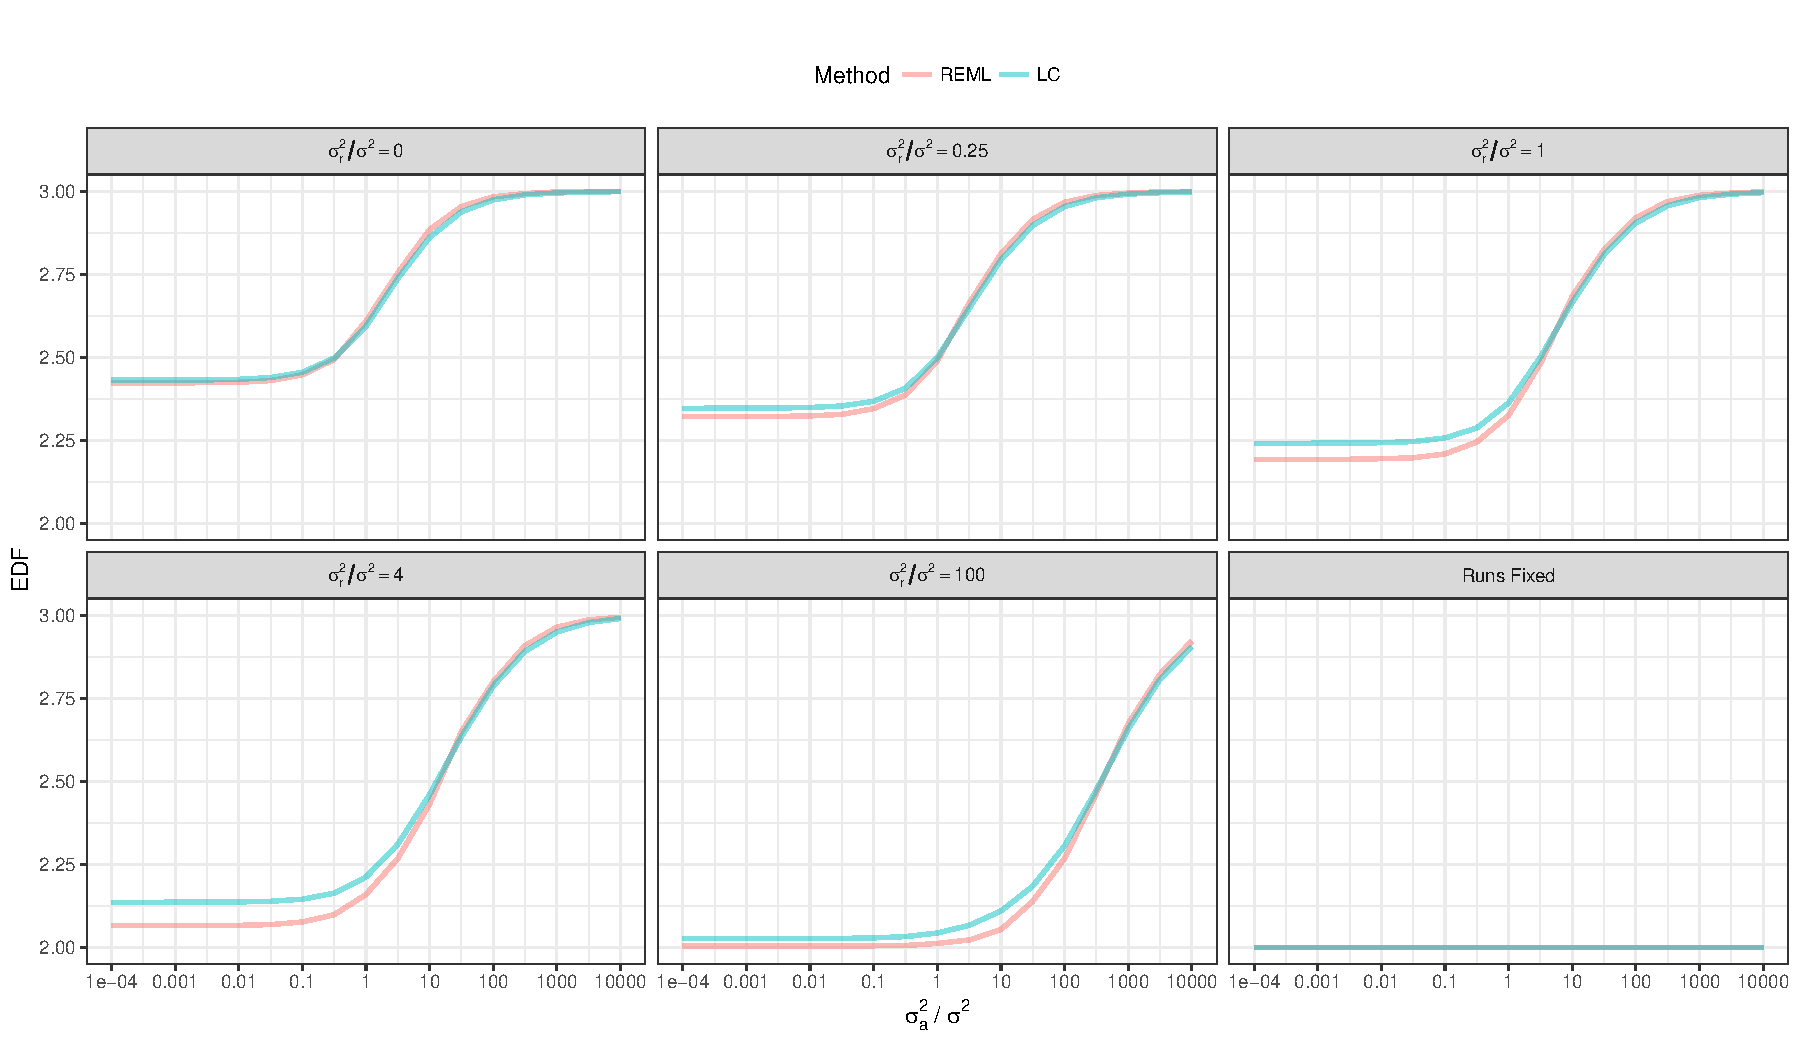
\includegraphics[width=1 \textwidth]{Chapter5/Graph/CRD232.pdf}
\caption{EDF for the variance of the treatment effects for two-phase experiment, i.e.\ for the optimal design of the Phase 2 experiment which takes account of the design of the Phase 1 experiment involves $\nu = 2$ treatments assigned to $n_a = 6$ animals. Each sample is further split into $n_s = 2$ sub-samples labelled by $n_\gamma = 4$ tags and measured in $n_r = 3$ runs, based on REML estimates of the variance components and on a linear combination of the mean squares.}
\label{fig:EDFadjusted}
\end{figure}

\section{EDF when Phase 1 experiment is arrange in a CRD}
\label{sec:expCRD}
This section compares the EDF obtained from optimal designs of the Phase 2 experiment found when the Phase 1 experiment is arranged in a CRD. The main consideration is on comparing four-plex and eight-plex experiments using an identical Phase 1 experiment. Three different cases are presented, showing that different sets of design parameters can work better depending on whether the four-plex or eight-plex experiment is used.

\subsection{Example 1: A CRD with 2 treatments and 12 animals}
The first example experiment to be considered is the Phase 1 experiment with $\nu = 2$ treatments assigned to $n_a = 12$ animals. Based on the methods presented in Chapter 3, two optimal designs are found for the Phase 2 proteomics experiment: one assuming the four-plex iTRAQ$^{\rm TM}$ system is used and the other assuming that the eight-plex system is used, which are presented in Tables~\ref{tab:aniDes1EDF} and \ref{tab:aniDes2EDF}, respectively.

\begin{table}[ht]
\centering   
\itshape 
\caption{Optimal (a) four- and (b) eight-plex designs of Phase 2 proteomics experiment when the Phase~1 experiment consists of $\nu = 2$ treatments assigned to each of $n_a = 12$ animals, with $n_s = 2$ sub-samples taken from each animal and analysed in the Phase 2 MudPIT-iTRAQ$^{\rm TM}$ experiment. Animal IDs are denoted by upper case letters, while the lower case letters a and b denote the two treatments.}
\begin{subtable}{.35 \linewidth} 
\caption{Four-plex system.}  
\begin{tabular}{c|cc:cc}
 & \multicolumn{4}{c}{{\bf Tag}} \\
{\bf Run}  & \textnormal{114} & \textnormal{115} & \textnormal{116} & \textnormal{117} \\ 
\hline  
\textnormal{1} & Jb & Aa & Lb & Ca \\ 
\textnormal{2} & Aa & Jb & Ca & Lb \\ 
\textnormal{3} & Ia & Fb & Hb & Ka \\ 
\textnormal{4} & Fb & Ia & Ka & Hb \\ 
\textnormal{5} & Bb & Ea & Db & Ga \\ 
\textnormal{6} & Ea & Bb & Ga & Db \\
\end{tabular} 
\label{tab:aniDes1EDF}
\end{subtable} 
\begin{subtable}{.5 \linewidth}   
\caption{Eight-plex system.}  
\begin{tabular}[t]{c|cc:cc:cc:cc}
 & \multicolumn{8}{c}{{\bf Tag}} \\
{\bf Run}  &  \textnormal{113} &  \textnormal{114} &  \textnormal{115} &  \textnormal{116} &  \textnormal{117} &  \textnormal{118} &  \textnormal{119} &  \textnormal{121}\\ \hline 
\textnormal{1} & Ia & Ea & Ga & Db & Hb & Ca & Bb & Jb \\ 
\textnormal{2} & Ea & Ia & Db & Ga & Ca & Hb & Jb & Bb \\ 
\textnormal{3} & Fb & Fb & Lb & Lb & Ka & Ka & Aa & Aa \\  
\end{tabular} 
\label{tab:aniDes2EDF}
\end{subtable}
\end{table}

The theoretical ANOVA tables for the four- and eight-plex optimal designs are presented in Tables~\ref{tab:ANOVAPhase1CRD11} and \ref{tab:ANOVAPhase1CRD12}, respectively. Based solely on these two theoretical ANOVA tables, the four-plex design is shown to be the better design, because it has higher Residual DF for estimating the Residual MS and therefore for testing treatment effects (7 DF compared to with 6 DF for the eight-plex design), and Treatment effects are fully estimated in the desired stratum, namely Between Animals within Runs. In comparison, the average efficiency factor for treatment effects in the eight-plex design is 0.889 due to the 1 DF of treatment contrast being partially confounded with the contrast of Tag 113, 114, 117, 118 versus Tag 115, 116, 119, 121. In addition, the theoretical ANOVA table of the four-plex experiment shows there are 2 DF associated with the residual variance in the Between Animals Between Runs stratum, potentially enabling the recovery of up to 2 additional DF, i.e.\ yielding up to 9 EDF. The eight-plex experiment has 1 DF associated with the Between Animals Between Runs stratum, which can be recovered giving EDF as high as 7 DF.  

\begin{table}[!ht]
\centering
 \caption{Theoretical ANOVA table for the optimal design of the Phase 2 experiment in Table~\ref{tab:aniDes1EDF}.}
 \begin{tabular}[t]{lrlll} 
 \toprule 
 \multicolumn{1}{l}{\textbf{Source of Variation}} & \multicolumn{1}{l}{\textbf{DF}} & \multicolumn{1}{l}{\textbf{EMS}}& \multicolumn{1}{l}{$\bm{E_{\gamma}}$}&\multicolumn{1}{l}{$\bm{E_{\tau}}$}\\ 
 \midrule 
 Between Runs &  &  & & \\ 
 \quad Between Animals & $2$ & $\sigma^2+2\sigma_{a}^2+4\sigma_{r}^2$ & & \\  \quad Within Animals & $3$ & $\sigma^2+4\sigma_{r}^2$ & & \\ \hline 
 Within Runs &  &  & & \\ 
 \quad Between Animals &  &  & & \\ 
 \quad \quad Tag & $1$ & $\sigma^2+2\sigma_{a}^2+6\theta_{\gamma}$ &$1$ & \\ 
 \quad \quad Treatment & $1$ & $\sigma^2+2\sigma_{a}^2+12\theta_{\tau}$ & & $1$\\ 
 \quad \quad Residual & $7$ & $\sigma^2+2\sigma_{a}^2$ & & \\ \hline 
 \quad Within Animals &  &  & & \\ 
 \quad \quad Tag & $2$ & $\sigma^2+6\theta_{\gamma}$ &$1$ & \\ 
 \quad \quad Residual & $7$ & $\sigma^2$ & & \\ 
 \bottomrule 
 \end{tabular} 
 \label{tab:ANOVAPhase1CRD11} 

\centering
 \caption{Theoretical ANOVA table for the optimal design of Phase 2 experiment in Table~\ref{tab:aniDes2EDF}.}
 \begin{tabular}[t]{lrlll} 
 \toprule 
 \multicolumn{1}{l}{\textbf{Source of Variation}} & \multicolumn{1}{l}{\textbf{DF}} & \multicolumn{1}{l}{\textbf{EMS}}& \multicolumn{1}{l}{$\bm{E_{\gamma}}$}&\multicolumn{1}{l}{$\bm{E_{\tau}}$}\\ 
 \midrule 
 Between Runs &  &  & & \\ 
 \quad Between Animals & $1$ & $\sigma^2+2\sigma_{a}^2+8\sigma_{r}^2$ & & \\  \quad Within Animals & $1$ & $\sigma^2+8\sigma_{r}^2$ & & \\ \hline 
 Within Runs &  &  & & \\ 
 \quad Between Animals &  &  & & \\ 
 \quad \quad Tag & $3$ & $\sigma^2+2\sigma_{a}^2+3\theta_{\gamma}+ 1.33\theta_{\tau}$ &$1$ & $0.1111$\\ 
 \quad \quad Treatment & $1$ & $\sigma^2+2\sigma_{a}^2+10.67\theta_{\tau}$ & & $0.8889$\\ 
 \quad \quad Residual & $6$ & $\sigma^2+2\sigma_{a}^2$ & & \\ \hline 
 \quad Within Animals &  &  & & \\ 
 \quad \quad Tag & $4$ & $\sigma^2+3\theta_{\gamma}$ &$1$ & \\ 
 \quad \quad Residual & $7$ & $\sigma^2$ & & \\ 
 \bottomrule 
 \end{tabular} 
 \label{tab:ANOVAPhase1CRD12} 
\end{table} 

\begin{figure}[!ht]
\centering
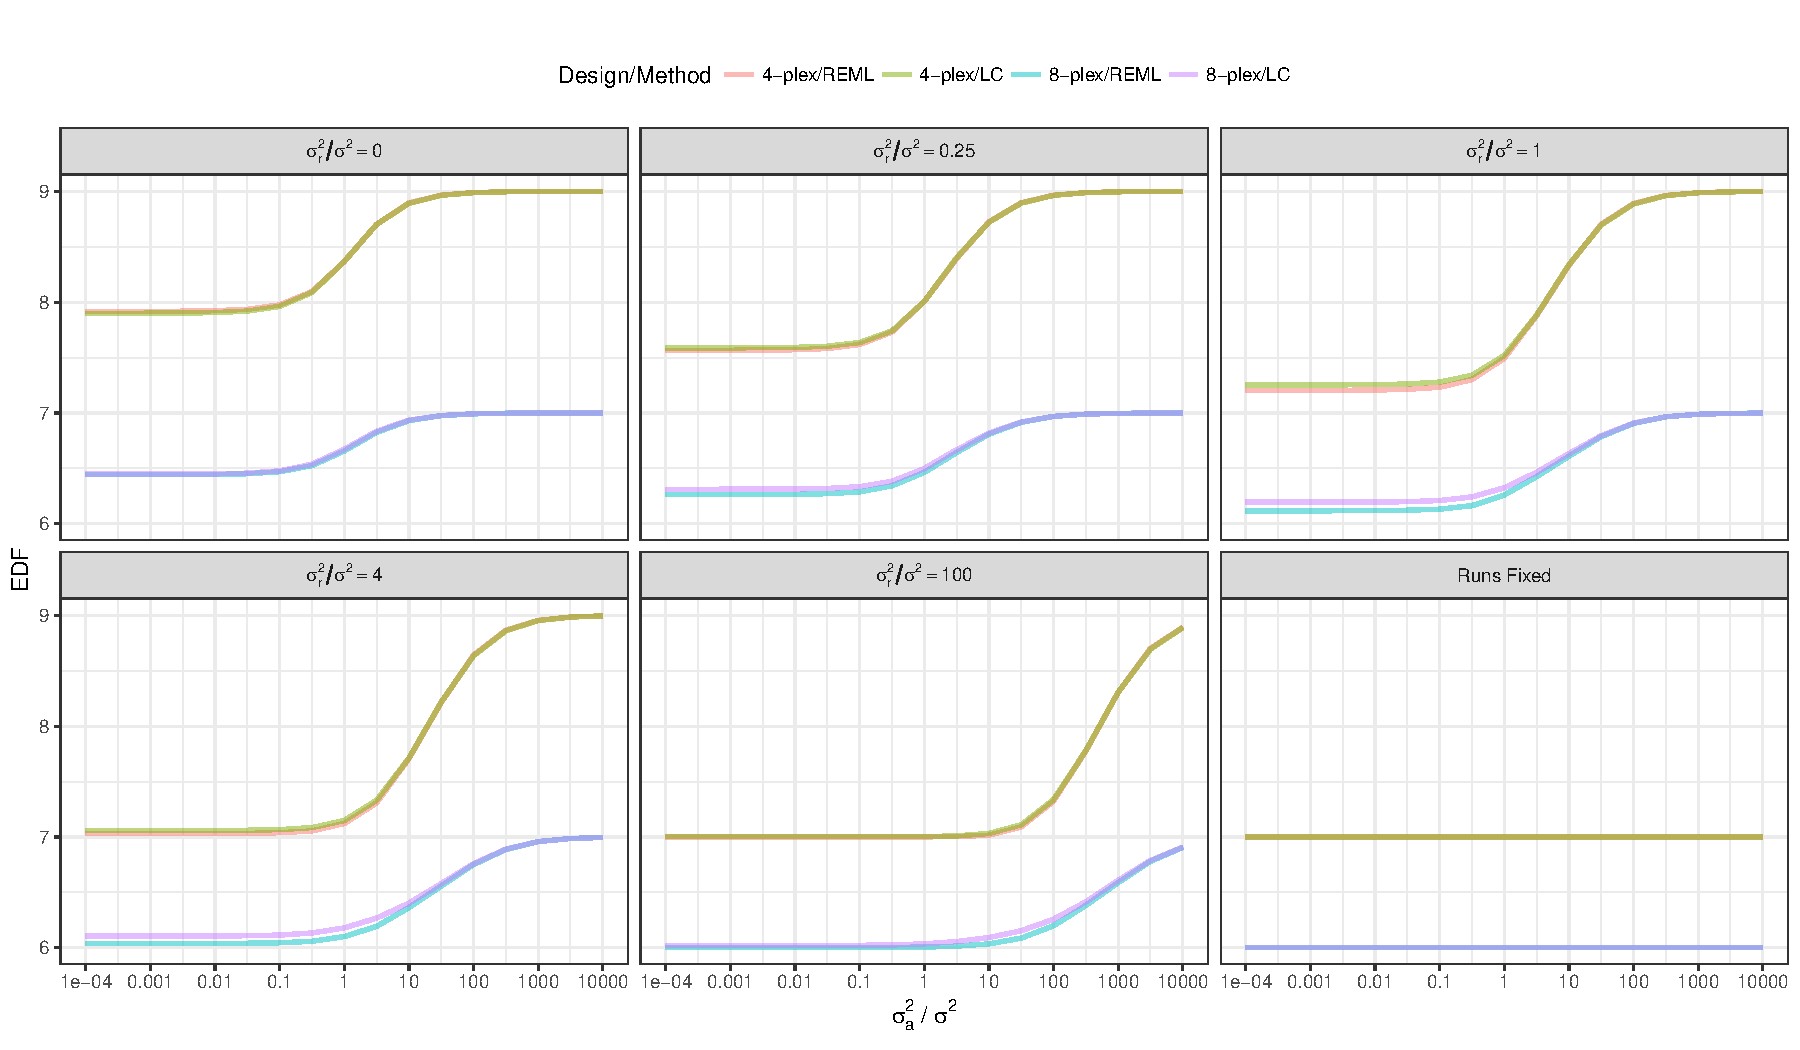
\includegraphics[width=1 \textwidth]{Chapter5/Graph/CRD262.pdf}
\caption{EDF plots for optimal designs shown in Tables~\ref{tab:aniDes1EDF} and \ref{tab:aniDes2EDF}, where EDF is calculated using VCs estimated by both the REML and LC methods.}
\label{fig:compare48CRD1}
\end{figure}

The EDF plots, in Figure~\ref{fig:compare48CRD1}, show that the EDF from the four-plex experiment is always higher than that from the  eight-plex experiment. The EDF of the four-plex experiment can be as low as 7 DF when there is large run-to-run variation, but the EDF approach 9 when the between-animal variation dominates. As for the eight-plex experiment, the EDF can be as low as 6 DF with large Run effects, but the EDF approach 7 with high between-animal variation. This suggests that the optimal design using the four-plex experiment is to be preferred over the eight-plex experiment in this case. In addition, the EDF appears to be very similar between the REML and LC methods.

\subsection{Example 2: A CRD with 8 treatments and 16 animals}
The second example experiment to be considered is a Phase 1 experiment with $\nu = 8$ treatments each assigned to $n_a = 16$ animals. Based on the methods presented in Chapter 3, two optimal designs are found for the Phase 2 proteomics experiment: one assuming the four-plex iTRAQ$^{\rm TM}$ system is used and the other assuming that the eight-plex system is used. These designs are presented in Tables~\ref{tab:aniDes3EDF} and \ref{tab:aniDes4EDF}, respectively.

\begin{table}[!ht]
\centering   
\itshape 
\caption{Optimal (a) four- and (b) eight-plex designs of Phase 2 proteomics experiment when the Phase~1 experiment consists of $\nu = 8$ treatments each assigned to $n_a = 16$ animals, with $n_s = 2$ sub-samples are then taken from each animal and analysed in the Phase 2 MudPIT-iTRAQ$^{\rm TM}$ experiment. Upper case letters denote animal IDs, while the lower case letters denote the treatments.}
\begin{subtable}{.35 \linewidth} 
\caption{Four-plex system.}  
\begin{tabular}{c|cc:cc}
 & \multicolumn{4}{c}{{\bf Tag}} \\
{\bf Run}  & \textnormal{114} & \textnormal{115} & \textnormal{116} & \textnormal{117} \\ 
\hline  
\textnormal{1} & Jb & Dd & Ph & Kc \\ 
\textnormal{2} & Dd & Jb & Kc & Ph \\ \hdashline
\textnormal{3} & Hh & Ee & Nf & Bb \\ 
\textnormal{4} & Ee & Hh & Bb & Nf \\ \hdashline
\textnormal{5} & Aa & Og & Me & Ld \\ 
\textnormal{6} & Og & Aa & Ld & Me \\ \hdashline
\textnormal{7} & Ff & Cc & Ia & Gg \\ 
\textnormal{8} & Cc & Ff & Gg & Ia \\ 
\end{tabular} 
\label{tab:aniDes3EDF}
\end{subtable} 
\begin{subtable}{.5 \linewidth}   
\caption{Eight-plex system.}  
\begin{tabular}[t]{c|cc:cc:cc:cc}
 & \multicolumn{8}{c}{{\bf Tag}} \\
{\bf Run}  &  \textnormal{113} &  \textnormal{114} &  \textnormal{115} &  \textnormal{116} &  \textnormal{117} &  \textnormal{118} &  \textnormal{119} &  \textnormal{121}\\ \hline 
\textnormal{1} & Ff & Dd & Kc & Hh & Me & Aa & Og & Bb \\ 
\textnormal{2} & Dd & Ff & Hh & Kc & Aa & Me & Bb & Og \\ \hdashline
\textnormal{3} & Cc & Ia & Nf & Jb & Gg & Ph & Ld & Ee \\ 
\textnormal{4} & Ia & Cc & Jb & Nf & Ph & Gg & Ee & Ld \\ 
\end{tabular} 
\label{tab:aniDes4EDF}
\end{subtable} 
\end{table}

The theoretical ANOVA tables for the four- and eight-plex optimal designs in Tables~\ref{tab:aniDes3EDF} and ~\ref{tab:aniDes4EDF} are presented in Tables~\ref{tab:ANOVAPhaseCRD31} and \ref{tab:ANOVAPhaseCRD32}, respectively. Based solely on these two theoretical ANOVA tables, both designs have the 4 Residual DF for estimating the Residual MS and therefore for testing Treatment effects. Furthermore, in both designs the Treatment effects are estimated, in the desired stratum, namely Between Animals within Runs, and have average efficiency factor \ $E_\tau = 0.8077$. 

For the four-plex experiment, the treatment average efficiency factor of $0.8077$ is due to the 3 DF associated with Treatment effects being confounded with Run effects. Thus, the Between Animals Between Runs EMS, which in previous cases provided a measure of pure error, now includes a contribution from the Treatment fixed effect. The 3 DF associated with this effect are not available for recovery of information, i.e. the existing 4 Residual DF for estimating the variance of the treatment effects cannot be improved upon. In comparison, although the treatment average efficiency factor, in the eight-plex design, is also $0.8077$, 3 of 7 DF associated with Treatment effects are now partially confounded with Tag effects. As a result, the 1 DF associated with the Between Animals MS in the Between Runs stratum remains pure error and can be recovered in the estimation of the VCs, resulting in the EDF to being as high as 5 DF. 


%thus, the mean square containing both the Between Animals VC, $\sigma_a^2$, and Between Runs VCs, $\sigma_r^2$, has to be regarded as fixed. Consequently, it is impossible to recover these 3 DF using the method presented in this Chapter. Therefore, the EDF for the four-plex experiment are always 4 DF.

\begin{table}[!ht]
\centering
 \caption{Theoretical ANOVA table for the optimal design of Phase 2 experiment in Table~\ref{tab:aniDes3EDF}.}
 \begin{tabular}[t]{lrlll} 
 \toprule 
 \multicolumn{1}{l}{\textbf{Source of Variation}} & \multicolumn{1}{l}{\textbf{DF}} & \multicolumn{1}{l}{\textbf{EMS}}& \multicolumn{1}{l}{$\bm{E_{\gamma}}$}&\multicolumn{1}{l}{$\bm{E_{\tau}}$}\\ 
 \midrule 
 Between Runs &  &  & & \\ 
 \quad Between Animals &  &  & & \\ 
 \quad \quad Treatment & $3$ & $\sigma^2+2\sigma_{a}^2+4\sigma_{r}^2+1.2\theta_{\tau}$ & & $0.3$\\ 
 \quad Within Animals & $4$ & $\sigma^2+4\sigma_{r}^2$ & & \\ \hline 
 Within Run &  &  & & \\ 
 \quad Between Animals &  &  & & \\ 
 \quad \quad Tag & $1$ & $\sigma^2+2\sigma_{a}^2+8\theta_{\gamma}$ &$1$ & \\ 
 \quad \quad Treatment & $7$ & $\sigma^2+2\sigma_{a}^2+ 3.23\theta_{\tau}$ & & $0.8077$\\ 
 \quad \quad Residual & $4$ & $\sigma^2+2\sigma_{a}^2$ & & \\ \hline 
 \quad Within Animals &  &  & & \\ 
 \quad \quad Tag & $2$ & $\sigma^2+8\theta_{\gamma}$ &$1$ & \\ 
 \quad \quad Residual & $10$ & $\sigma^2$ & & \\ 
 \bottomrule 
 \end{tabular} 
 \label{tab:ANOVAPhaseCRD31} 

 \caption{Theoretical ANOVA table for the optimal design of Phase 2 experiment in Table~\ref{tab:aniDes4EDF}.}
 \begin{tabular}[t]{lrlll} 
 \toprule 
 \multicolumn{1}{l}{\textbf{Source of Variation}} & \multicolumn{1}{l}{\textbf{DF}} & \multicolumn{1}{l}{\textbf{EMS}}& \multicolumn{1}{l}{$\bm{E_{\gamma}}$}&\multicolumn{1}{l}{$\bm{E_{\tau}}$}\\ 
 \midrule 
 Between Runs &  &  & & \\ 
 \quad Between Animals & $1$ & $\sigma^2+2\sigma_{a}^2+8\sigma_{r}^2$ & & \\ 
 \quad Within Animals & $2$ & $\sigma^2+8\sigma_{r}^2$ & & \\ \hline 
 Within Runs &  &  & & \\ 
 \quad Between Animals &  &  & & \\ 
 \quad \quad Tag & $3$ & $\sigma^2+2\sigma_{a}^2+4\theta_{\gamma}+1.2\theta_{\tau}$ &$1$ &  $0.3$\\ 
 \quad \quad Treatment & $7$ & $\sigma^2+2\sigma_{a}^2+3.23\theta_{\tau}$ & & $0.8077$\\ 
 \quad \quad Residual & $4$ & $\sigma^2+2\sigma_{a}^2$ & & \\ \hline 
 \quad Within Animals &  &  & & \\ 
 \quad \quad Tag & $4$ & $\sigma^2+4\theta_{\gamma}$ &$1$ & \\ 
 \quad \quad Residual & $10$ & $\sigma^2$ & & \\ 
 \bottomrule 
 \end{tabular} 
 \label{tab:ANOVAPhaseCRD32} 
\end{table} 

The EDF plots, in Figure~\ref{fig:compare82CRD}, show that the EDF for the design using the eight-plex system is always 4 irrespective of the values of the ratios $\sigma_a^2/\sigma^2$ and $\sigma_r^2/\sigma^2$. For the four-plex design, the EDF can be as low as 4 when the run-to-run variation is much larger than the between animal variation, and as high as 5 DF when the between-animal variation dominates. The EDF are the same (4 DF) between four- and eight-plex experiments when $\sigma_r^2/\sigma^2 = 100$ and $\sigma_a^2/\sigma^2$ is between $1 \times 10^{-4}$ to $10$, i.e.\ when the run-to-run  variation is 10 to $1 \times 10^{6}$ times of run-to-run variation over animal-to-animal variation. The EDF are also the same (4 DF) between four- and eight-plex experiments when Run effects are assumed to be fixed. In addition, the EDF are again shown to be very similar between the REML and LC methods.

\begin{figure}[!ht]
\centering
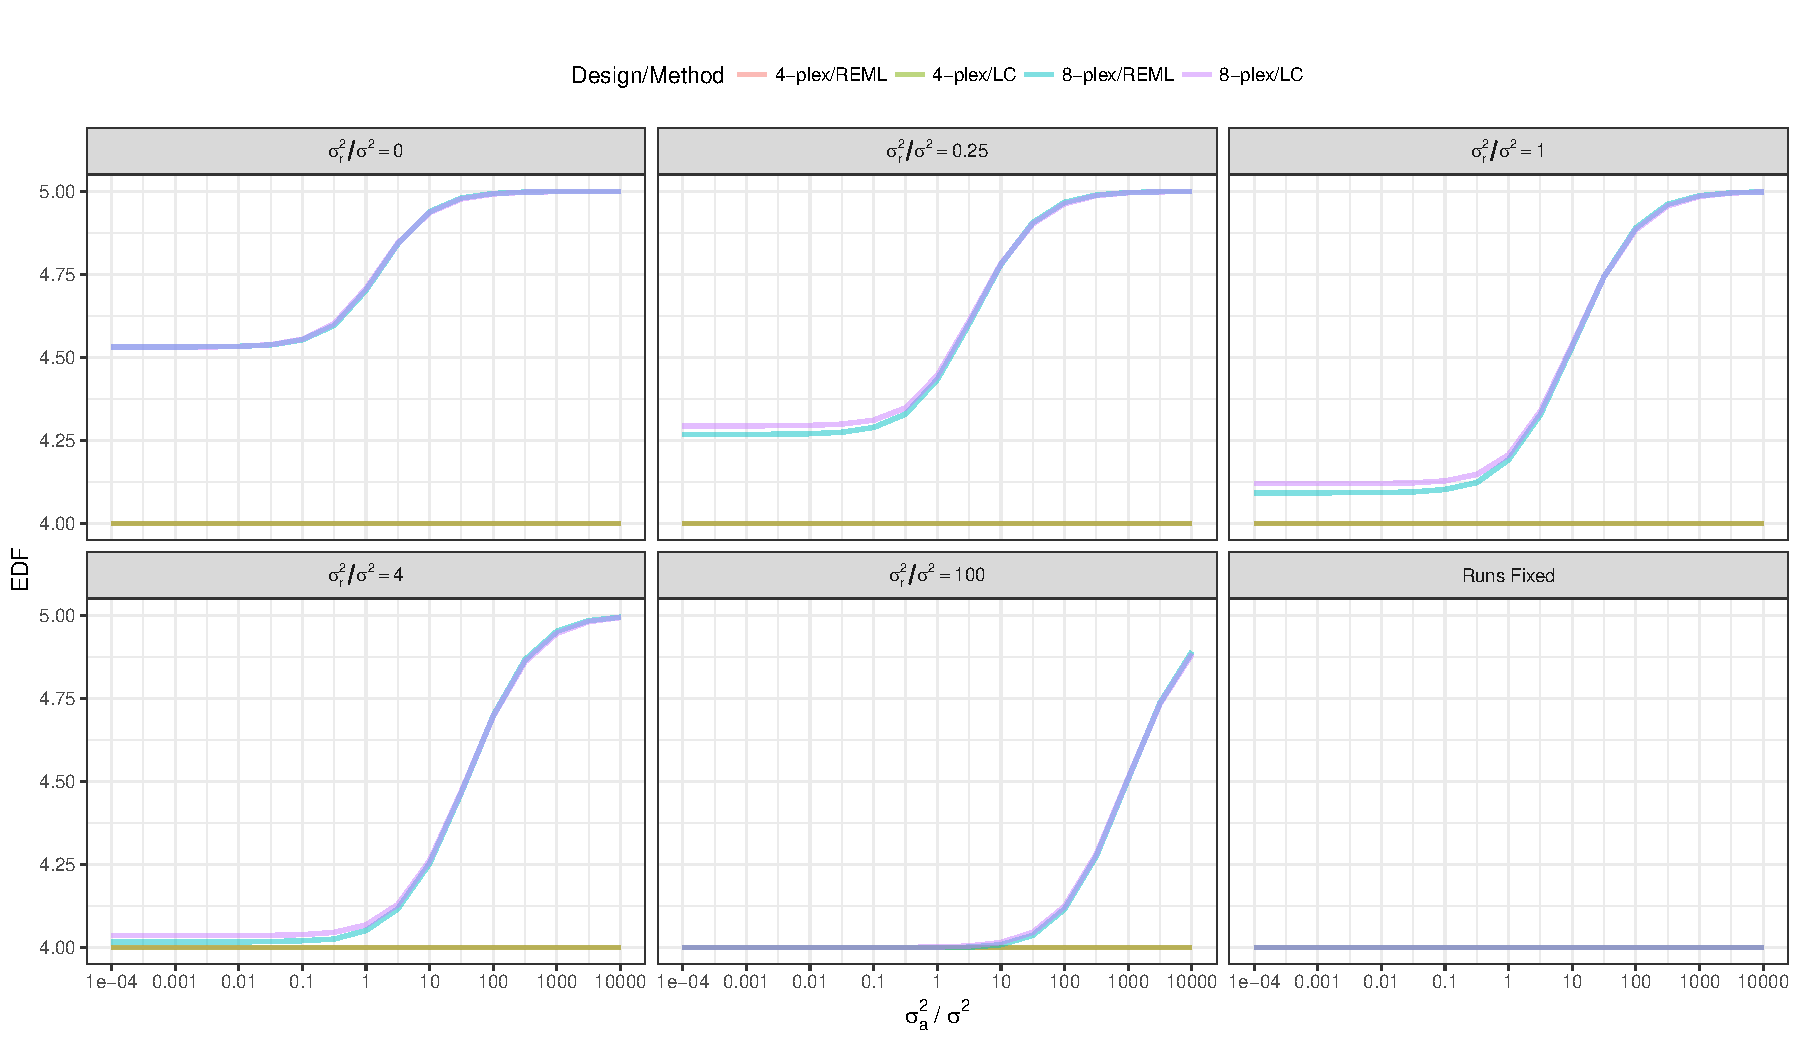
\includegraphics[width=1 \textwidth]{Chapter5/Graph/CRD822.pdf}
\caption{EDF plots for optimal designs shown in Tables~\ref{tab:aniDes3EDF} and \ref{tab:aniDes4EDF}, where EDF is calculated using VCs estimated by both the REML and LC methods.}
\label{fig:compare82CRD}
\end{figure}

\subsection{Example 3: A CRD with 4 treatments and 24 animals}
In the third example, the Phase 1 experiment involves $\nu = 4$ treatments assigned to $n_a = 24$ animals. Based on the methods presented in Chapter 3, two optimal designs are found for the Phase 2 proteomics experiment: one assuming the four-plex iTRAQ$^{\rm TM}$ system is used and the other assuming that the eight-plex system is used. These designs are presented in Tables~\ref{tab:aniDes5EDF} and \ref{tab:aniDes6EDF}, respectively.

\begin{table}[ht]
\centering
\itshape
\caption{Optimal (a) four- and (b) eight-plex designs of Phase 2 proteomics experiment, when the Phase~1 experiment consists of $\nu = 4$ treatments assigned to each of $n_a = 24$ animals, $n_s = 2$ sub-samples are then taken from each animal and analysed in the Phase 2 MudPIT-iTRAQ$^{\rm TM}$ experiment. Upper case letters denote animal IDs, while the lower case letters denote the treatments.}
\begin{subtable}{.35 \linewidth} 
\caption{Four-plex system.}  
\begin{tabular}{c|cc:cc}
 & \multicolumn{4}{c}{{\bf Tag}} \\
{\bf Run}  & \textnormal{114} & \textnormal{115} & \textnormal{116} & \textnormal{117} \\ 
\hline  
\textnormal{1} & Aa & Rb & Cc & Dd \\ 
\textnormal{2}  2 & Rb & Aa & Dd & Cc \\ \hdashline
\textnormal{3}  3 & Ea & Fb & Gc & Hd \\ 
\textnormal{4}  4 & Fb & Ea & Hd & Gc \\ \hdashline
\textnormal{5}  5 & Ia & Jb & Kc & Ld \\ 
\textnormal{6}  6 & Jb & Ia & Ld & Kc \\ \hdashline
\textnormal{7}  7 & Oc & Pd & Ma & Nb \\ 
\textnormal{8}  8 & Pd & Oc & Nb & Ma \\ \hdashline
\textnormal{9}  9 & Sc & Td & Qa & Bb \\ 
\textnormal{10}  10 & Td & Sc & Bb & Qa \\ \hdashline
\textnormal{11}  11 & Wc & Xd & Ua & Vb \\ 
\textnormal{12}  12 & Xd & Wc & Vb & Ua \\ 
\end{tabular} 
\label{tab:aniDes5EDF}
\end{subtable} 
\begin{subtable}{.5 \linewidth}   
\caption{Eight-plex system.} 
\begin{tabular}[t]{c|cc:cc:cc:cc}
 & \multicolumn{8}{c}{{\bf Tag}} \\
{\bf Run}  &  \textnormal{113} &  \textnormal{114} &  \textnormal{115} &  \textnormal{116} &  \textnormal{117} &  \textnormal{118} &  \textnormal{119} &  \textnormal{121}\\ \hline 
\textnormal{1} & Vb & Ma & Qa & Pd & Dd & Wc & Bb & Oc \\ 
\textnormal{2} & Ma & Vb & Pd & Qa & Wc & Dd & Oc & Bb \\ \hdashline
\textnormal{3} & Kc & Rb & Td & Cc & Jb & Ea & Aa & Hd \\ 
\textnormal{4} & Rb & Kc & Cc & Td & Ea & Jb & Hd & Aa \\ \hdashline
\textnormal{5} & Sc & Ld & Fb & Nb & Xd & Ua & Gc & Ia \\ 
\textnormal{6} & Ld & Sc & Nb & Fb & Ua & Xd & Ia & Gc \\ 
\end{tabular} 
\label{tab:aniDes6EDF}
\end{subtable} 
\end{table}

The theoretical ANOVA tables for the four- and eight-plex optimal designs in Tables~\ref{tab:aniDes5EDF} and \ref{tab:aniDes6EDF} are presented in Tables~\ref{tab:ANOVAPhase1CRD21} and \ref{tab:ANOVAPhase1CRD22}, respectively. Based solely on these two theoretical ANOVA tables, the eight-plex design  has higher Residual DF for estimating the Residual MS and for testing treatment effects (15 DF compared 14 DF for the four-plex design). Comparing the treatment average efficiency factor from the two designs: $E_\tau = 0.9623$ for the eight-plex design which is slightly lower than $E_\tau =1$ for the four-plex design. In addition, the theoretical ANOVA table of the four-plex design has 5 DF associated with the Between Animals Between Runs stratum, which can be recovered giving EDF as high as 19, whereas the eight-plex experiment has 2 DF associated with the Between Animals Between Runs stratum, which can be recovered giving EDF as high as 17.  

\begin{table}[!ht]
\centering
 \caption{Theoretical ANOVA table for the optimal design of Phase 2 experiment in Table~\ref{tab:aniDes5EDF}.}
 \begin{tabular}[t]{lrlll} 
 \toprule 
 \multicolumn{1}{l}{\textbf{Source of Variation}} & \multicolumn{1}{l}{\textbf{DF}} & \multicolumn{1}{l}{\textbf{EMS}}& \multicolumn{1}{l}{$\bm{E_{\gamma}}$}&\multicolumn{1}{l}{$\bm{E_{\tau}}$}\\ 
 \midrule 
 Between Runs &  &  & & \\ 
 \quad Between Animals & $5$ & $\sigma^2+2\sigma_{a}^2+4\sigma_{r}^2$ & & \\  \quad Within Animals & $6$ & $\sigma^2+4\sigma_{r}^2$ & & \\ \hline 
 Within Runs &  &  & & \\ 
 \quad Between Animals &  &  & & \\ 
 \quad \quad Tag & $1$ & $\sigma^2+2\sigma_{a}^2+12\theta_{\gamma}$ &$1$ & \\ 
 \quad \quad Treatment & $3$ & $\sigma^2+2\sigma_{a}^2+12\theta_{\tau}$ & & $1$\\ 
 \quad \quad Residual & $14$ & $\sigma^2+2\sigma_{a}^2$ & & \\ \hline 
 \quad Within Animals &  &  & & \\ 
 \quad \quad Tag & $2$ & $\sigma^2+12\theta_{\gamma}$ &$1$ & \\ 
 \quad \quad Residual & $16$ & $\sigma^2$ & & \\ 
 \bottomrule 
 \end{tabular} 
 \label{tab:ANOVAPhase1CRD21} 

 \caption{Theoretical ANOVA table for the optimal design of Phase 2 experiment in Table~\ref{tab:aniDes6EDF}.}
 \begin{tabular}[t]{lrlll} 
 \toprule 
 \multicolumn{1}{l}{\textbf{Source of Variation}} & \multicolumn{1}{l}{\textbf{DF}} & \multicolumn{1}{l}{\textbf{EMS}}& \multicolumn{1}{l}{$\bm{E_{\gamma}}$}&\multicolumn{1}{l}{$\bm{E_{\tau}}$}\\ 
 \midrule 
 Between Runs &  &  & & \\ 
 \quad Between Animals & $2$ & $\sigma^2+2\sigma_{a}^2+8\sigma_{r}^2$ & & \\  \quad Within Animals & $3$ & $\sigma^2+8\sigma_{r}^2$ & & \\ \hline 
 Within Runs &  &  & & \\ 
 \quad Between Animals &  &  & & \\ 
 \quad \quad Tag & $3$ & $\sigma^2+2\sigma_{a}^2+6\theta_{\gamma}+ 0.67\theta_{\tau}$ &$1$ & $0.0556$\\ 
 \quad \quad Treatment & $3$ & $\sigma^2+2\sigma_{a}^2+11.55\theta_{\tau}$ & & $0.9623$\\ 
 \quad \quad Residual & $15$ & $\sigma^2+2\sigma_{a}^2$ & & \\ \hline 
 \quad Within Animals &  &  & & \\ 
 \quad \quad Tag & $4$ & $\sigma^2+6\theta_{\gamma}$ &$1$ & \\ 
 \quad \quad Residual & $17$ & $\sigma^2$ & & \\ 
 \bottomrule 
 \end{tabular} 
 \label{tab:ANOVAPhase1CRD22} 
\end{table} 

\begin{figure}[!h]
\centering
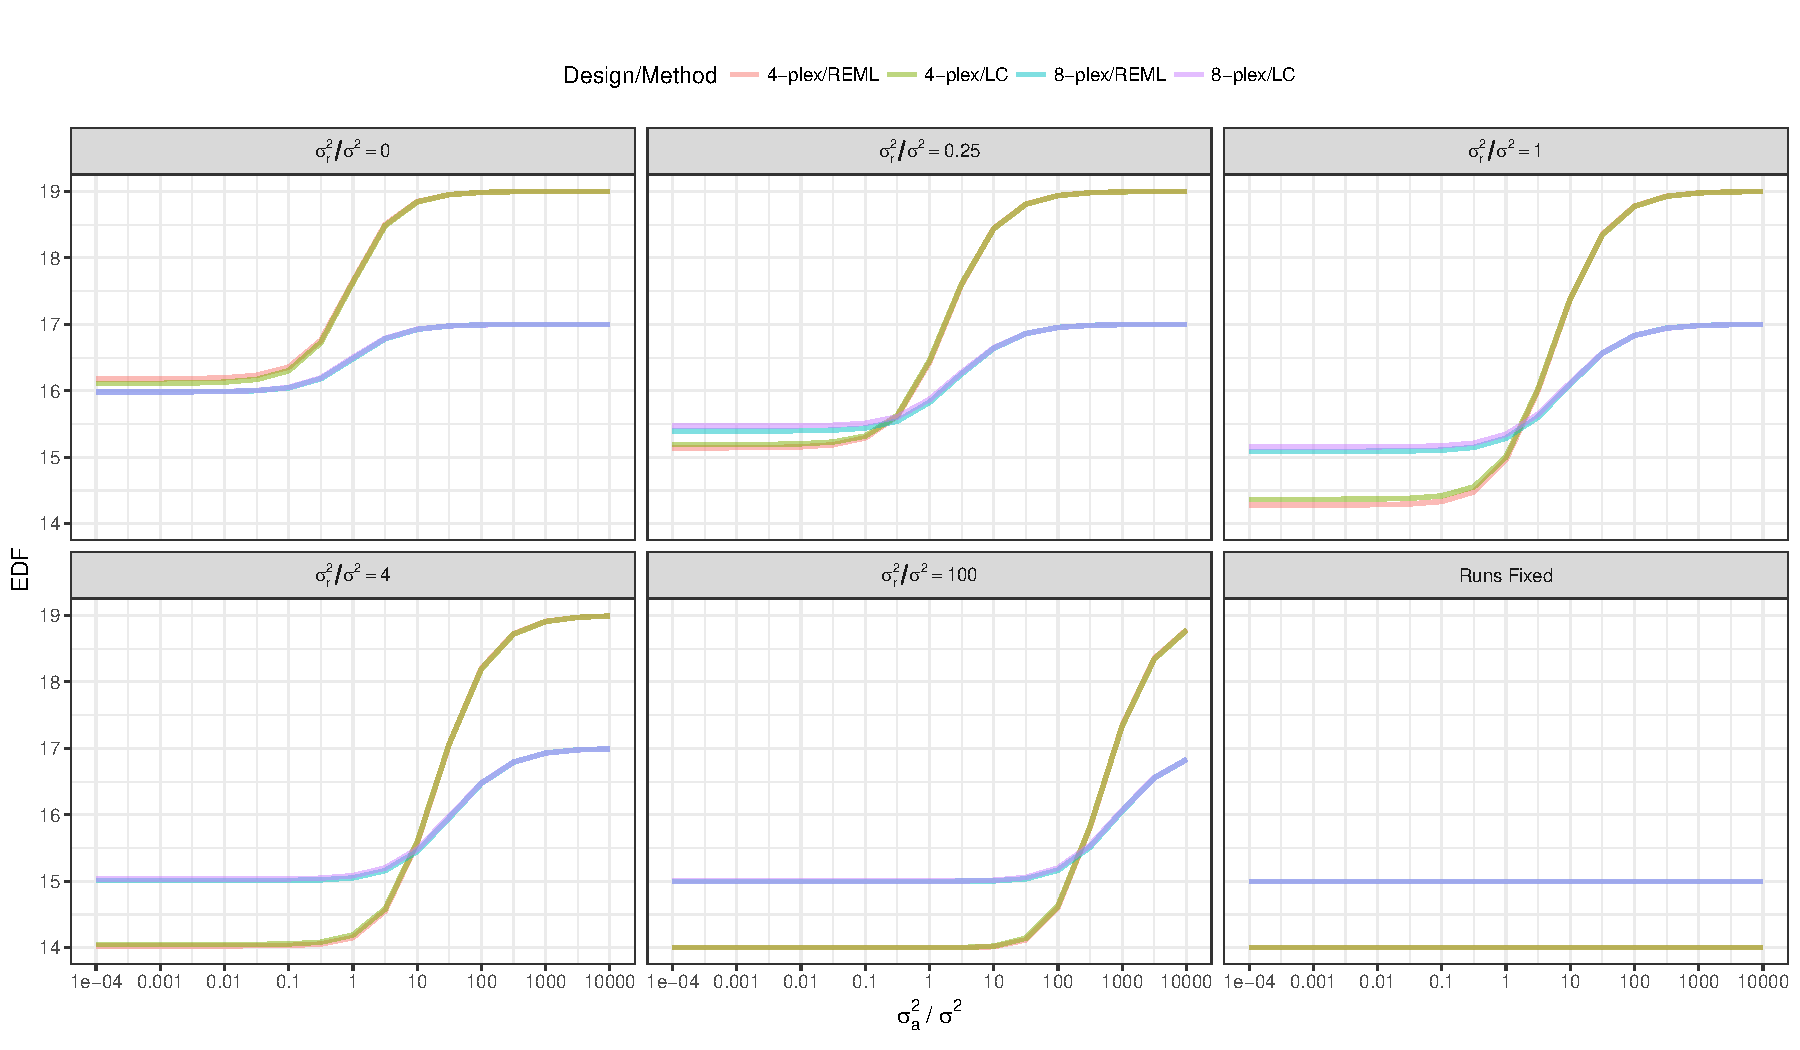
\includegraphics[width=1 \textwidth]{Chapter5/Graph/CRD462.pdf}
\caption{EDF plots for optimal designs shown in Tables~\ref{tab:aniDes5EDF} and \ref{tab:aniDes6EDF}, where EDF is calculated using VCs estimated by both the REML and LC methods.}
\label{fig:compare44CRD}
\end{figure}

The EDF plots, in Figure~\ref{fig:compare44CRD}, show that, for the design using the four-plex experiment, the EDF can be as low as 14 when the run-to-run variation is much larger than the between-animal variation, and as high as 19 when between-animal variation dominates. For the the design using eight-plex experiment, the EDF can be as low as 15 DF when the run-to-run variation is much larger than the between-animal variation, and as high as 17 DF when the between-animal variation dominates. Furthermore, recall from the theoretical ANOVA tables (in Tables~\ref{tab:ANOVAPhase1CRD21} and \ref{tab:ANOVAPhase1CRD22}) that the eight-plex design has 15 Residual DF compared with 14 Residual DF in the four-plex design. From the EDF plots, we can see the EDF for the four-plex design exceed those of the eight-plex design as $\sigma_a^2/\sigma^2$ increases. For example, when $\sigma_r^2/\sigma^2 = 0.25$, the EDF become higher for the four-plex experiment when $\sigma_a^2/\sigma^2 = 1 \times 10^{-0.5}$, that is about $0.79$ times of the run-to-run variation over animal-to-animal variation. Table~\ref{tab:edfCompare} lists the $\sigma_r^2/\sigma^2$ and $\sigma_a^2/\sigma^2$ combinations when the EDF become higher for the four-plex experiment than the eight-plex experiment, and the magnitudes of the run-to-run variation over animal-to-animal variation based on Figure~\ref{fig:compare44CRD}. 

\begin{table}[!h]
\centering
\caption{Magnitudes of the run-to-run variation over animal-to-animal variation when the EDF become higher for four-plex experiment than eight-plex experiments based on Figure~\ref{fig:compare44CRD}.}
\begin{tabular}{|c|l|l|l|l|}
\hline 
$\sigma_r^2/\sigma^2$ 	& $0.25$ & $1$ & $4$ & $100$ \\ 
\hline 
$\sigma_a^2/\sigma^2$ 	& $10^{-0.5}$ & $10^{0.25}$ & $10$ & $10^{2.25}$ \\ 
\hline 
$\sigma_r^2/\sigma_a^2$ 	 & $0.79$ & $0.56$ & $0.4$ & $0.32$ \\ 
\hline 
\end{tabular} 
\label{tab:edfCompare}
\end{table}

% When $\sigma_r^2/\sigma^2 = 1$, the EDF become higher for four-plex experiment when $\sigma_a^2/\sigma^2 = 1 \times 10^{0.25}$, that is about $0.56$ times of the run-to-run variation over animal-to-animal variation. When $\sigma_r^2/\sigma^2 = 4$, the EDF become higher for four-plex experiment when $\sigma_a^2/\sigma^2 = 10$, that is about $0.4$ times of the run-to-run variation over animal-to-animal variation. Finally, when $\sigma_r^2/\sigma^2 = 100$, the EDF become higher for four-plex experiment when $\sigma_a^2/\sigma^2 = 1 \times 10^{2.25}$, that is about $0.32$ times of the run-to-run variation over animals to animal variation. In addition, the EDF again shown to be not different between the REML and LC methods.


\section{Comparing the EDF when Phase 1 experiment is arranged in a RCBD}
\label{sec:expRCBD}
This section compares the EDF of optimal designs between Phase 2 four-plex and eight-plex experiments when the Phase 1 experiment is arranged in a RCBD. There are four types of designs that can be compared, given the same Phase 1 experiment is arranged in a RCBD: 
\begin{enumerate}
\item Phase 1 Block effects are intentionally confounded with Run effects using the four-plex system,
\item Phase 1 Block effects are intentionally confounded with Tag effects using the four-plex system,
\item Phase 1 Block effects are intentionally confounded with Run effects using the eight-plex system and
\item Phase 1 Block effects are intentionally confounded with Tag effects using the eight-plex system,
\end{enumerate}
The same method for estimating the VCs and approximating the EDF can also be applied to this example, because we can still construct an ANOVA table with Residual MS which assumed to have a chi-square distribution. In addition, the EDF are still approximated based on the Residual MS of the Between Experimental units (Plants) Within Blocks (Trays) Within Runs stratum, i.e.\ $\sigma^2 + \sigma_p^2$.

This section first compares designs from two different confounding schemes for each four- and eight-plex experiment, followed by an overall comparison between the four- and eight-plex systems. The Phase 2 experiment uses plants as an example when the Phase 1 experiment involves $\nu = 4$ treatments assigned to $n_p = 16$ plants in $n_b = 4$ trays. Then $n_s = 2$ sub-samples are obtained from each plant, i.e.\ a total of 32 sub-samples, for the Phase 2 proteomics experiment.  

The simulation study was done on the basis that MS has at chi-square distribution, with the ratio of Between Plants VCs to measurement error, denoted by $\sigma_p^2/\sigma^2$, set with 17 values ranging from $10^{-4}$ to $10^4$, the ratio of Between Trays VCs to measurement error and Between Runs VCs to measurement error, denoted by $\sigma_b^2/\sigma^2$ and $\sigma_r^2/\sigma^2$, respectively, set to $0, 0.25, 1, 5, 100$, as well as having effects of tray and run fixed are also considered (effectively when $\sigma _b^2 = \infty$ and $\sigma _r^2 = \infty$). 

\subsection{Four-plex system}
Given the Phase 1 experiment with $\nu = 4$ treatments assigned to $n_a = 16$ plants in $n_b = 4$ trays, based on the methods presented in Chapter 4, two optimal designs are found for the Phase 2 four-plex proteomics experiment: one assumes that Tray effects are intentionally confounded with Run effects, and the other that Tray effects are intentionally confounded with Tag effects. These are presented in Tables~\ref{tab:aniDes5EDF} and \ref{tab:aniDes6EDF}, respectively.

\begin{table}[!ht]
\centering   
\itshape 
\caption{Optimal design of Phase 2 proteomics experiment showing allocation of sub-samples from trays, plants and treatments to runs and tags, when the Phase~1 experiment consists of $\nu = 2$ treatments assigned to $n_a = 16$ plants in $n_b = 4$ trays, $n_s = 2$ sub-samples are then taken from each plant and analysed in the Phase 2 MudPIT-iTRAQ$^{\rm TM}$ experiment using $n_\gamma = 4$ tags. Numbers denote trays, upper case letters denote plant IDs, while the lower case letters denote the treatments.}
\begin{subtable}{.35 \linewidth} 
\caption{Tray effects are intentionally confounded with Run effects.}  
\begin{tabular}{c|cc:cc}
 & \multicolumn{4}{c}{{\bf Tag}} \\
{\bf Run}  & \textnormal{114} & \textnormal{115} & \textnormal{116} & \textnormal{117} \\ 
\hline  
\textnormal{1} & 1Cc & 1Dd & 1Bb & 1Aa \\ 
\textnormal{2} & 1Dd & 1Cc & 1Aa & 1Bb \\ \hdashline
\textnormal{3} & 2Hd & 2Fb & 2Ea & 2Gc \\ 
\textnormal{4} & 2Fb & 2Hd & 2Gc & 2Ea \\ \hdashline
\textnormal{5} & 3Ia & 3Jb & 3Ld & 3Kc \\ 
\textnormal{6} & 3Jb & 3Ia & 3Kc & 3Ld \\ \hdashline
\textnormal{7} & 4Ma & 4Oc & 4Pd & 4Nb \\ 
\textnormal{8} & 4Oc & 4Ma & 4Nb & 4Pd \\ 
\end{tabular} 
\label{tab:aniTrayDes1EDF}
\end{subtable} 
\begin{subtable}{.35 \linewidth}   
\caption{Tray effects are intentionally confounded with Tag effects.}  
\begin{tabular}{c|cc:cc}
 & \multicolumn{4}{c}{{\bf Tag}} \\
{\bf Run}  & \textnormal{114} & \textnormal{115} & \textnormal{116} & \textnormal{117} \\ 
\hline  
\textnormal{1} & 1Bb & 1Dd & 3Kc & 3Ia \\ 
\textnormal{2} & 1Dd & 1Bb & 3Ia & 3Kc \\ 
\textnormal{3} & 1Cc & 1Aa & 3Ld & 3Jb \\ 
\textnormal{4} & 1Aa & 1Cc & 3Jb & 3Ld \\ \hdashline
\textnormal{5} & 2Gc & 2Fb & 4Ma & 4Pd \\ 
\textnormal{6} & 2Fb & 2Gc & 4Pd & 4Ma \\ 
\textnormal{7} & 2Ea & 2Hd & 4Nb & 4Oc \\ 
\textnormal{8} & 2Hd & 2Ea & 4Oc & 4Nb \\ 
\end{tabular} 
\label{tab:aniTrayDes2EDF}
\end{subtable} 
\end{table}

The theoretical ANOVA tables for the optimal designs of the Phase 2 experiment using the four-plex system are presented in Tables~\ref{tab:ANOVAPhase1RCBD1} and \ref{tab:ANOVAPhase1RCBD2}, respectively. Based solely on these two theoretical ANOVA tables, the design when Tray effects are intentionally confounded with Run effects is shown to be the better design, because it has higher Residual DF for estimating the Residual MS and therefore for testing Treatment effects (8 DF compared to 7 DF for the four-plex design) in the Between Plants Within Trays stratum. Both designs can estimate Treatment effects with full efficiency in the Between Plants Within Trays stratum, because the treatment average efficiency factors for both designs are 100\%. 

From the theoretical ANOVA of both designs, there is extra information on the Between Plants VC $\sigma_{p}^2$ in the Between Trays Between Runs MS, however, we may not be able to recover this information, because we cannot equate Residual MS in Between Trays Between Runs stratum based on the EMS to estimate $\sigma_{p}^2$. For the design when the Tray effects are intentionally confounded the Run effects (see Table~\ref{tab:ANOVAPhase1RCBD2}), there are 2 DF associated with the Between Plants Within Blocks Between Runs stratum which can be recovered giving EDF as high as 9.  

\begin{table}[!ht]
\centering
 \caption{Theoretical ANOVA table from the Phase 2 experiment in Table~\ref{tab:aniTrayDes1EDF}.}
 \begin{tabular}[t]{lrlll} 
 \toprule 
 \multicolumn{1}{l}{\textbf{Source of Variation}} & \multicolumn{1}{l}{\textbf{DF}} & \multicolumn{1}{l}{\textbf{EMS}}& \multicolumn{1}{l}{$\bm{E_{\gamma}}$}&\multicolumn{1}{l}{$\bm{E_{\tau}}$}\\ 
 \midrule 
 Between Runs &  &  & & \\ 
 \quad Between Trays & $3$ & $\sigma^2+2\sigma_{p}^2+8\sigma_{b}^2+4\sigma_{r}^2$ & & \\  
 \quad Within Plants Within Trays & $4$ & $\sigma^2+4\sigma_{r}^2$ & & \\ \hline 
 Within Runs &  &  & & \\ 
 \quad Between Plants Within Trays &  &  & & \\ 
 \quad \quad Tag & $1$ & $\sigma^2+2\sigma_{p}^2+8\theta_{\gamma}$ &$1$ & \\ 
 \quad \quad Treatment & $3$ & $\sigma^2+2\sigma_{p}^2+8\theta_{\tau}$ & & $1$\\ 
 \quad \quad Residual & $8$ & $\sigma^2+2\sigma_{p}^2$ & & \\ \hline 
 \quad Within Plants Within Trays &  &  & & \\ 
 \quad \quad Tag & $2$ & $\sigma^2+8\theta_{\gamma}$ &$1$ & \\ 
 \quad \quad Residual & $10$ & $\sigma^2$ & & \\ 
 \bottomrule 
 \end{tabular} 
 \label{tab:ANOVAPhase1RCBD1} 

 \caption{Theoretical ANOVA table from the Phase 2 experiment in Table~\ref{tab:aniTrayDes2EDF}.}
 \begin{tabular}[t]{lrlll} 
 \toprule 
 \multicolumn{1}{l}{\textbf{Source of Variation}} & \multicolumn{1}{l}{\textbf{DF}} & \multicolumn{1}{l}{\textbf{EMS}}& \multicolumn{1}{l}{$\bm{E_{\gamma}}$}&\multicolumn{1}{l}{$\bm{E_{\tau}}$}\\ 
 \midrule 
 Between Runs &  &  & & \\ 
 \quad Between Trays & $1$ & $\sigma^2+2\sigma_{p}^2+8\sigma_{b}^2+4\sigma_{r}^2$ & & \\  
 \quad Between Plants Within Trays & $2$ & $\sigma^2+2\sigma_{p}^2+4\sigma_{r}^2$ & & \\  
 \quad Within Plants Within Trays & $4$ & $\sigma^2+4\sigma_{r}^2$ & & \\ \hline 
 Within Runs &  &  & & \\ 
 \quad Between Trays &  &  & & \\ 
 \quad \quad Tag & $1$ & $\sigma^2+2\sigma_{p}^2+8\sigma_{b}^2+8\theta_{\gamma}$ &$1$ & \\ 
 \quad \quad Residual & $1$ & $\sigma^2+2\sigma_{p}^2+8\sigma_{b}^2$ & & \\ \hline 
 \quad Between Plants Within Trays &  &  & & \\ 
 \quad \quad Treatment & $3$ & $\sigma^2+2\sigma_{p}^2+8\theta_{\tau}$ & & $1$\\ 
 \quad \quad Residual & $7$ & $\sigma^2+2\sigma_{p}^2$ & & \\ \hline 
 \quad Within Plants Within Trays &  &  & & \\ 
 \quad \quad Tag & $2$ & $\sigma^2+8\theta_{\gamma}$ &$1$ & \\ 
 \quad \quad Residual & $10$ & $\sigma^2$ & & \\ 
 \bottomrule 
 \end{tabular} 
 \label{tab:ANOVAPhase1RCBD2} 
\end{table} 

\begin{landscape}
\begin{figure}[h!]
\centering
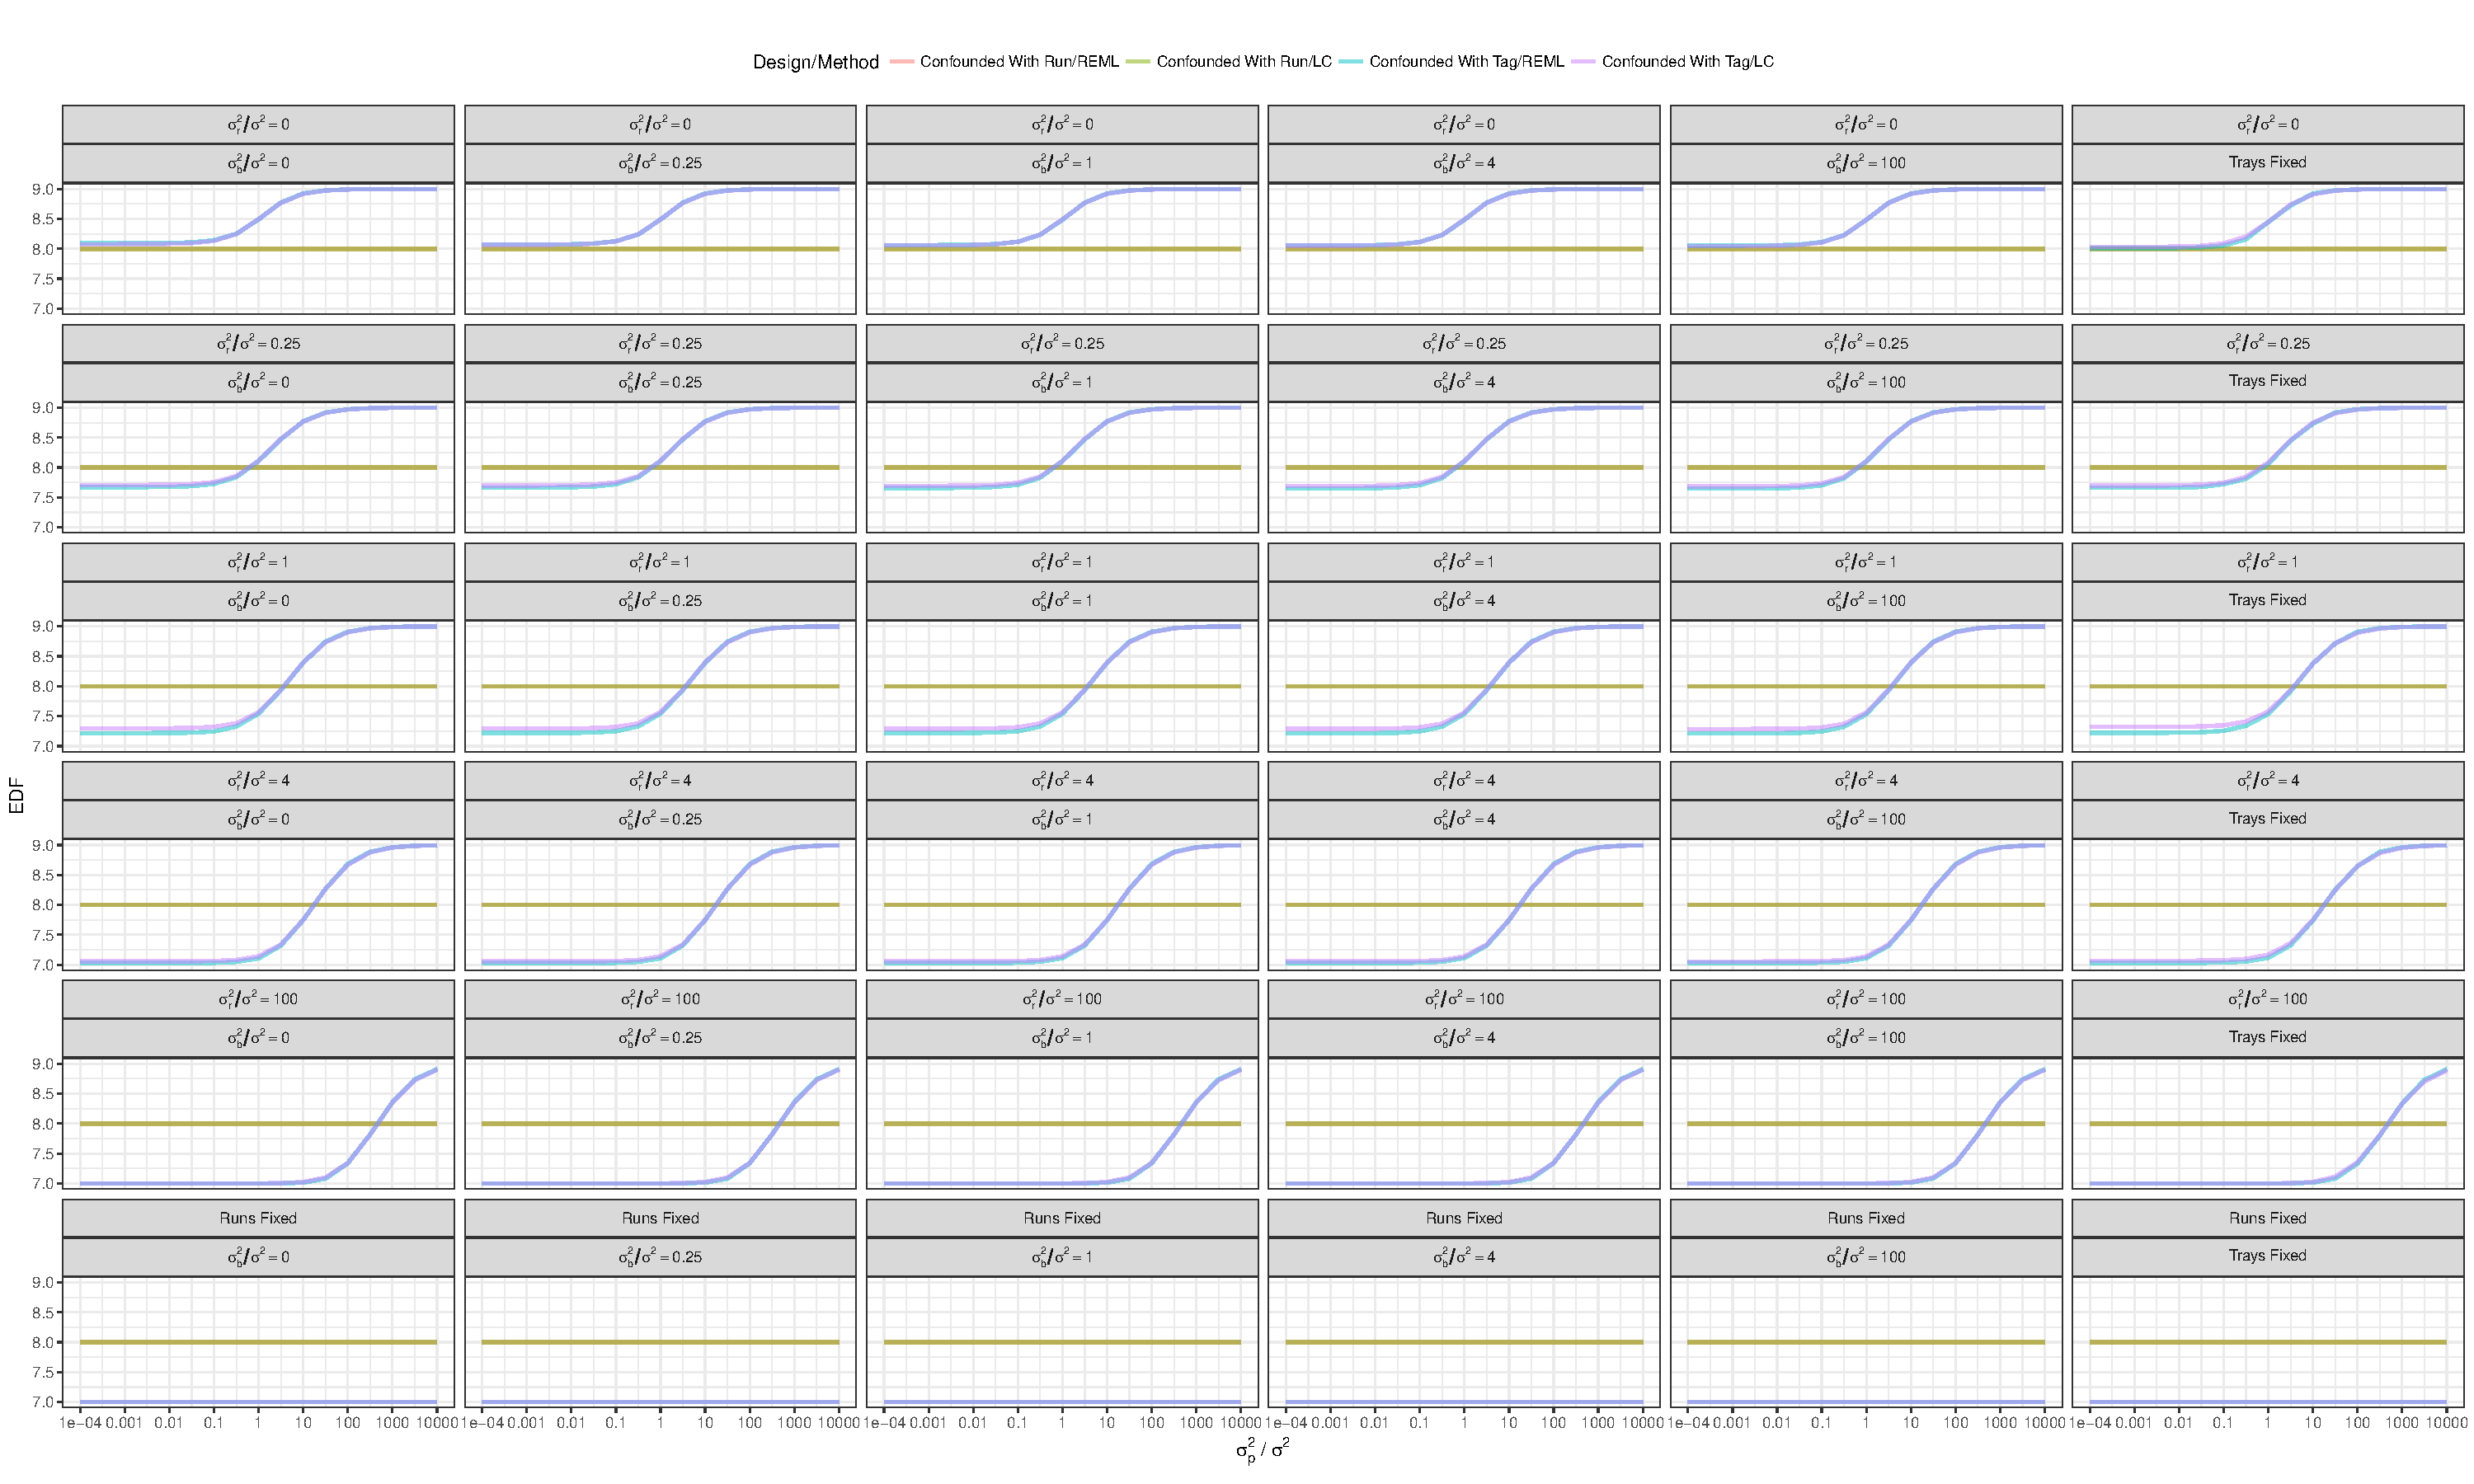
\includegraphics[width=1.3 \textwidth]{Chapter5/Graph/CRD44424.pdf}
\caption{EDF plots for optimal designs shown in Tables~\ref{tab:aniTrayDes1EDF} and \ref{tab:aniTrayDes2EDF}, where EDF is calculated using VCs estimated by both the REML and LC methods.}
\label{fig:RCBD442Tag4EDF}
\end{figure}
\end{landscape}

The EDF plots in Figure~\ref{fig:RCBD442Tag4EDF} are presented as a 6-by-6 panels having different combination of ranges of ratios for Between Plants VCs, Between Trays VCs and Between Runs VCs to measurement error, denoted by $\sigma_p^2/\sigma^2$, $\sigma_b^2/\sigma^2$ and $\sigma_r^2/\sigma^2$, respectively. We can first observe that different values of the ratio $\sigma_b^2/\sigma^2$ do not change the EDF. For the design when Tray effects are intentionally confounded with Run effects, the EDF are always 8 DF. For the design when Tray effects are intentionally confounded with Tag effects, the EDF can be as low as 7 DF when run-to-run variation is much larger than the between-plants variation, but the EDF approach 9 DF when the between-plants variation dominates. From the EDF plot, we can see that the EDF of the design when Tray effects are intentionally confounded with Tag effects become better than the design when Tray effects are intentionally confounded with Run effects as $\sigma_p^2/\sigma^2$ increases. For example, when $\sigma_r^2/\sigma^2 = 0.25$, the EDF become higher when $\sigma_p^2/\sigma^2 = 1$, that is about $0.25$ times of the run-to-run variation over plant-to-plant variation. Table~\ref{tab:edfCompare} lists the $\sigma_r^2/\sigma^2$ and $\sigma_p^2/\sigma^2$ combinations when the EDF become higher for the design when Tray effects are intentionally confounded with Tag effects than the design when Tray effects are intentionally confounded with Run effects, and the magnitudes of the run-to-run variation over plant-to-plant variation are based on Figure~\ref{fig:compare44CRD}. In addition, the EDF are again shown to be very similar between the REML and LC methods.

\begin{table}[!h]
\centering
\caption{Magnitudes of the run-to-run variation over plant-to-plant variation when the EDF become higher for design when Tray effects are intentionally confounded with Tag effects than the design when Tray effects are intentionally confounded with Run effect based on Figure~\ref{fig:RCBD442Tag4EDF}.}
\begin{tabular}{|c|l|l|l|l|}
\hline 
$\sigma_r^2/\sigma^2$ 	& $0.25$ & $1$ & $4$ & $100$ \\ 
\hline 
$\sigma_p^2/\sigma^2$ 	& $1$ & $ 10^{0.5}$ & $10^{1.25}$ & $10^{2.75}$ \\ 
\hline 
$\sigma_r^2/\sigma_p^2$ & $0.25$ & $0.32$ & $0.22$ & $0.18$ \\ 
\hline 
\end{tabular} 
\label{tab:edfCompare1}
\end{table}


%The example experiment to be considered features a Phase 1 experiment consisting of $\nu = 4$, $r_b = 4, n_B  = 4$ and $r_t = 2$. Four different two-phase designs can be compared using the same Phase 1 experiment. The theoretical ANOVA tables for each of these four designs are presented in Tables~\ref{tab:ANOVAPhase1RCBD1}, \ref{tab:ANOVAPhase1RCBD2}, \ref{tab:ANOVAPhase1RCBD3} and \ref{tab:ANOVAPhase1RCBD4}. Based on these four theoretical ANOVA tables, Tables~\ref{tab:ANOVAPhase1RCBD1} and \ref{tab:ANOVAPhase1RCBD4} appear to perform equally well, with the most residual DF of 8 and $100\%$ of the treatment information in the Between Plants Within Trays Within Runs stratum. The EDF are then assessed for each of these four designs. 


\subsection{Eight-plex system}
Using the same Phase 1 experiment with $\nu = 4$ treatments assigned to $n_a = 16$ plants in $n_b = 4$ trays, there are two optimal design that are found in the Phase 2 proteomics experiment using the eight-plex system. The first design assumes that the Tray effects are intentionally confounded with Run effects (see Tables~\ref{tab:aniDes5EDF}). The second design assumes that Tray effects are intentionally confounded with Tag effects (see Tables~\ref{tab:aniDes5EDF}).

\begin{table}[!ht]
\centering   
\itshape 
\caption{Optimal design of Phase 2 proteomics experiment showing allocation of sub-samples from trays, plants and treatments to runs and tags, when the Phase~1 experiment consists of $\nu = 2$ treatments assigned to $n_a = 16$ plants in $n_b = 4$ trays, $n_s = 2$ sub-samples are then taken from each plant and analysed in the Phase 2 MudPIT-iTRAQ$^{\rm TM}$ experiment using $n_\gamma = 8$ tags. Numbers denote trays, upper case letters denote plant IDs, while the lower case letters denote the treatments.}
\begin{subtable}{.55 \linewidth} 
\caption{Tray effects are intentionally confounded with Run effects.}  
\begin{tabular}[t]{c|cccc:cccc}
 & \multicolumn{8}{c}{{\bf Tag}} \\
{\bf Run}  &  \textnormal{113} &  \textnormal{114} &  \textnormal{115} &  \textnormal{116} &  \textnormal{117} &  \textnormal{118} &  \textnormal{119} &  \textnormal{121}\\ \hline 
\textnormal{1} & 1Bb & 1Dd & 1Aa & 1Cc & 2Ea & 2Fb & 2Gc & 2Hd \\ 
\textnormal{2} & 1Dd & 1Bb & 1Cc & 1Aa & 2Fb & 2Ea & 2Hd & 2Gc \\ \hdashline
\textnormal{3} & 3Ia & 3Kc & 3Ld & 3Jb & 4Oc & 4Pd & 4Ma & 4Nb \\ 
\textnormal{4} & 3Kc & 3Ia & 3Jb & 3Ld & 4Pd & 4Oc & 4Nb & 4Ma \\ 
\end{tabular} 
\label{tab:aniTrayDes3EDF}
\end{subtable} 
\begin{subtable}{.55 \linewidth}   
\caption{Tray effects are intentionally confounded with Run effects.}  
\begin{tabular}[t]{c|cc:cc:cc:cc}
 & \multicolumn{8}{c}{{\bf Tag}} \\
{\bf Run}  &  \textnormal{113} &  \textnormal{114} &  \textnormal{115} &  \textnormal{116} &  \textnormal{117} &  \textnormal{118} &  \textnormal{119} &  \textnormal{121}\\ \hline 
\textnormal{1} & 1Aa & 1Cc & 2Gc & 2Fb & 3Ld & 3Ia & 4Pd & 4Nb \\ 
\textnormal{2} & 1Cc & 1Aa & 2Fb & 2Gc & 3Ia & 3Ld & 4Nb & 4Pd \\ \hdashline
\textnormal{3} & 1Bb & 1Dd & 2Hd & 2Ea & 3Kc & 3Jb & 4Ma & 4Oc \\ 
\textnormal{4} & 1Dd & 1Bb & 2Ea & 2Hd & 3Jb & 3Kc & 4Oc & 4Ma \\ 
\end{tabular} 
\label{tab:aniTrayDes4EDF}
\end{subtable} 
\end{table}

The theoretical ANOVA tables for the optimal designs of the Phase 2 experiment using the eight-plex system are presented in Tables~\ref{tab:ANOVAPhase1RCBD1} and \ref{tab:ANOVAPhase1RCBD2}, respectively. Based solely on these two theoretical ANOVA tables, the design when Tray effects are intentionally confounded with Tag effects is shown to be the better design, because it has higher Residual DF for estimating the Residual MS and therefore for testing Treatment effects (8 DF compared to 7 DF for the four-plex design) in the Between Plants Within Trays stratum. Both designs can estimate Treatment effects with full efficiency in the Between Plants Within Trays stratum, because the treatment average efficiency factors $E_\tau$ for both designs are 100\%. 

For the design in which the Tray effects are intentionally confounded with Run effects (see Table~\ref{tab:ANOVAPhase1RCBD3}), there is no extra information on the Between Plants VC $\sigma_{p}^2$ that can be recovered, because these $\sigma_{p}^2$ are all in Between Trays Between Runs MS and we cannot equate residual MS in the Between Trays Between Runs strata based on the EMS to estimate $\sigma_{p}^2$ for this design. 

For the design when the Tray effects are intentionally confounded with Tag effects (see Table~\ref{tab:ANOVAPhase1RCBD4}), there are 2 DF associated with the Between Plants Within Blocks Between Runs stratum which can be recovered giving EDF as high as 10 DF. In addition, since the 3 DF associated with Tray effects are confounded with Tag effects, Tray effects can only be considered to be fixed.       

\begin{table}[!ht]
\centering
 \caption{Theoretical ANOVA table of the Phase 2 experiment in Table~\ref{tab:aniTrayDes3EDF}.}
 \begin{tabular}[t]{lrlll} 
 \toprule 
 \multicolumn{1}{l}{\textbf{Source of Variation}} & \multicolumn{1}{l}{\textbf{DF}} & \multicolumn{1}{l}{\textbf{EMS}}& \multicolumn{1}{l}{$\bm{E_{\gamma}}$}&\multicolumn{1}{l}{$\bm{E_{\tau}}$}\\ 
 \midrule 
 Between Runs &  &  & & \\ 
 \quad Between Trays & $1$ & $\sigma^2+2\sigma_{p}^2+8\sigma_{b}^2+8\sigma_{r}^2$ & & \\  
 \quad Within Plants Within Trays & $2$ & $\sigma^2+8\sigma_{r}^2$ & & \\ \hline 
 Within Runs &  &  & & \\ 
 \quad Between Trays &  &  & & \\ 
 \quad \quad Tag & $1$ & $\sigma^2+2\sigma_{p}^2+8\sigma_{b}^2+4\theta_{\gamma}$ &$1$ & \\ 
 \quad \quad Residual & $1$ & $\sigma^2+2\sigma_{p}^2+8\sigma_{b}^2$ & & \\ \hline 
 \quad Between Plants Within Trays &  &  & & \\ 
 \quad \quad Tag & $2$ & $\sigma^2+2\sigma_{p}^2+4\theta_{\gamma}$ &$1$ & \\ 
 \quad \quad Treatment & $3$ & $\sigma^2+2\sigma_{p}^2+8\theta_{\tau}$ & & $1$\\ 
 \quad \quad Residual & $7$ & $\sigma^2+2\sigma_{p}^2$ & & \\ \hline 
 \quad Within Plants Within Trays &  &  & & \\ 
 \quad \quad Tag & $4$ & $\sigma^2+4\theta_{\gamma}$ &$1$ & \\ 
 \quad \quad Residual & $10$ & $\sigma^2$ & & \\ 
 \bottomrule 
 \end{tabular} 
 \label{tab:ANOVAPhase1RCBD3} 

 \caption{Theoretical ANOVA table of the Phase 2 experiment in Table~\ref{tab:aniTrayDes4EDF}.}
 \begin{tabular}[t]{lrlll} 
 \toprule 
 \multicolumn{1}{l}{\textbf{Source of Variation}} & \multicolumn{1}{l}{\textbf{DF}} & \multicolumn{1}{l}{\textbf{EMS}}& \multicolumn{1}{l}{$\bm{E_{\gamma}}$}&\multicolumn{1}{l}{$\bm{E_{\tau}}$}\\ 
 \midrule 
 Between Runs &  &  & & \\ 
 \quad Between Plants Within Trays & $1$ & $\sigma^2+2\sigma_{p}^2+8\sigma_{r}^2$ & & \\ 
 \quad Within Plants Within Trays & $2$ & $\sigma^2+8\sigma_{r}^2$ & & \\ \hline 
 Within Runs &  &  & & \\ 
 \quad Between Trays &  &  & & \\ 
 \quad \quad Tag & $3$ & $\sigma^2+2\sigma_{p}^2+8\sigma_{b}^2+4\theta_{\gamma}$ &$1$ & \\ \hline 
 \quad Between Plants Within Trays &  &  & & \\ 
 \quad \quad Treatment & $3$ & $\sigma^2+2\sigma_{p}^2+8\theta_{\tau}$ & & $1$\\ 
 \quad \quad Residual & $8$ & $\sigma^2+2\sigma_{p}^2$ & & \\ \hline 
 \quad Within Plants Within Trays &  &  & & \\ 
 \quad \quad Tag & $4$ & $\sigma^2+4\theta_{\gamma}$ &$1$ & \\ 
 \quad \quad Residual & $10$ & $\sigma^2$ & & \\ 
 \bottomrule 
 \end{tabular} 
 \label{tab:ANOVAPhase1RCBD4} 
\end{table} 

%The first comparison of the EDF is between the two designs using the four-plex experiments using the EDF plots in Figure~\ref{fig:RCBD442Tag4EDF}. The design in which cages are confounded more with runs is indicated by the pink line for which the EDF are always 8. This phenomenon can be explained by the theoretical ANOVA table in Table~\ref{tab:ANOVAPhase1RCBD1}, where the Between Runs stratum does not contain the Between Plants Within Trays stratum. Another explanation is that the VCs estimates can only be derived from the Within Runs stratum. In Figure~\ref{fig:RCBD442Tag4EDF}, the remaining six colours represent the EDF with different VCs of Between Trays, these plots show the Between Trays VCs can only affect the EDF when the Between Plants VCs are small.  

The EDF plots, in Figure~\ref{fig:compare48CRD1}, show that the EDF for the design when the Tray effects are intentionally confounded with Run effects is always 7 DF under different ranges of values of the ratios $\sigma_p^2/\sigma^2$, $\sigma_b^2/\sigma^2$ and $\sigma_r^2/\sigma^2$. 

For the design when Tray effects are intentionally confounded with Tag effects, the change of EDF can only be observed when the Tray effects are assumed to be fixed. Further, the EDF can be as low as 8 DF when run-to-run variation is much larger than the between-plants variation, but the EDF approach 9 DF when the between plants variation dominates. Therefore, the design in which Tray effects are intentionally confounded with Tag effects is always better than the design in which the Tray effects are intentionally confounded with Run effects using the eight-plex system. The EDF are again shown to be very similar between the REML and LC methods.

\begin{landscape}
\begin{figure}[h!]
\centering
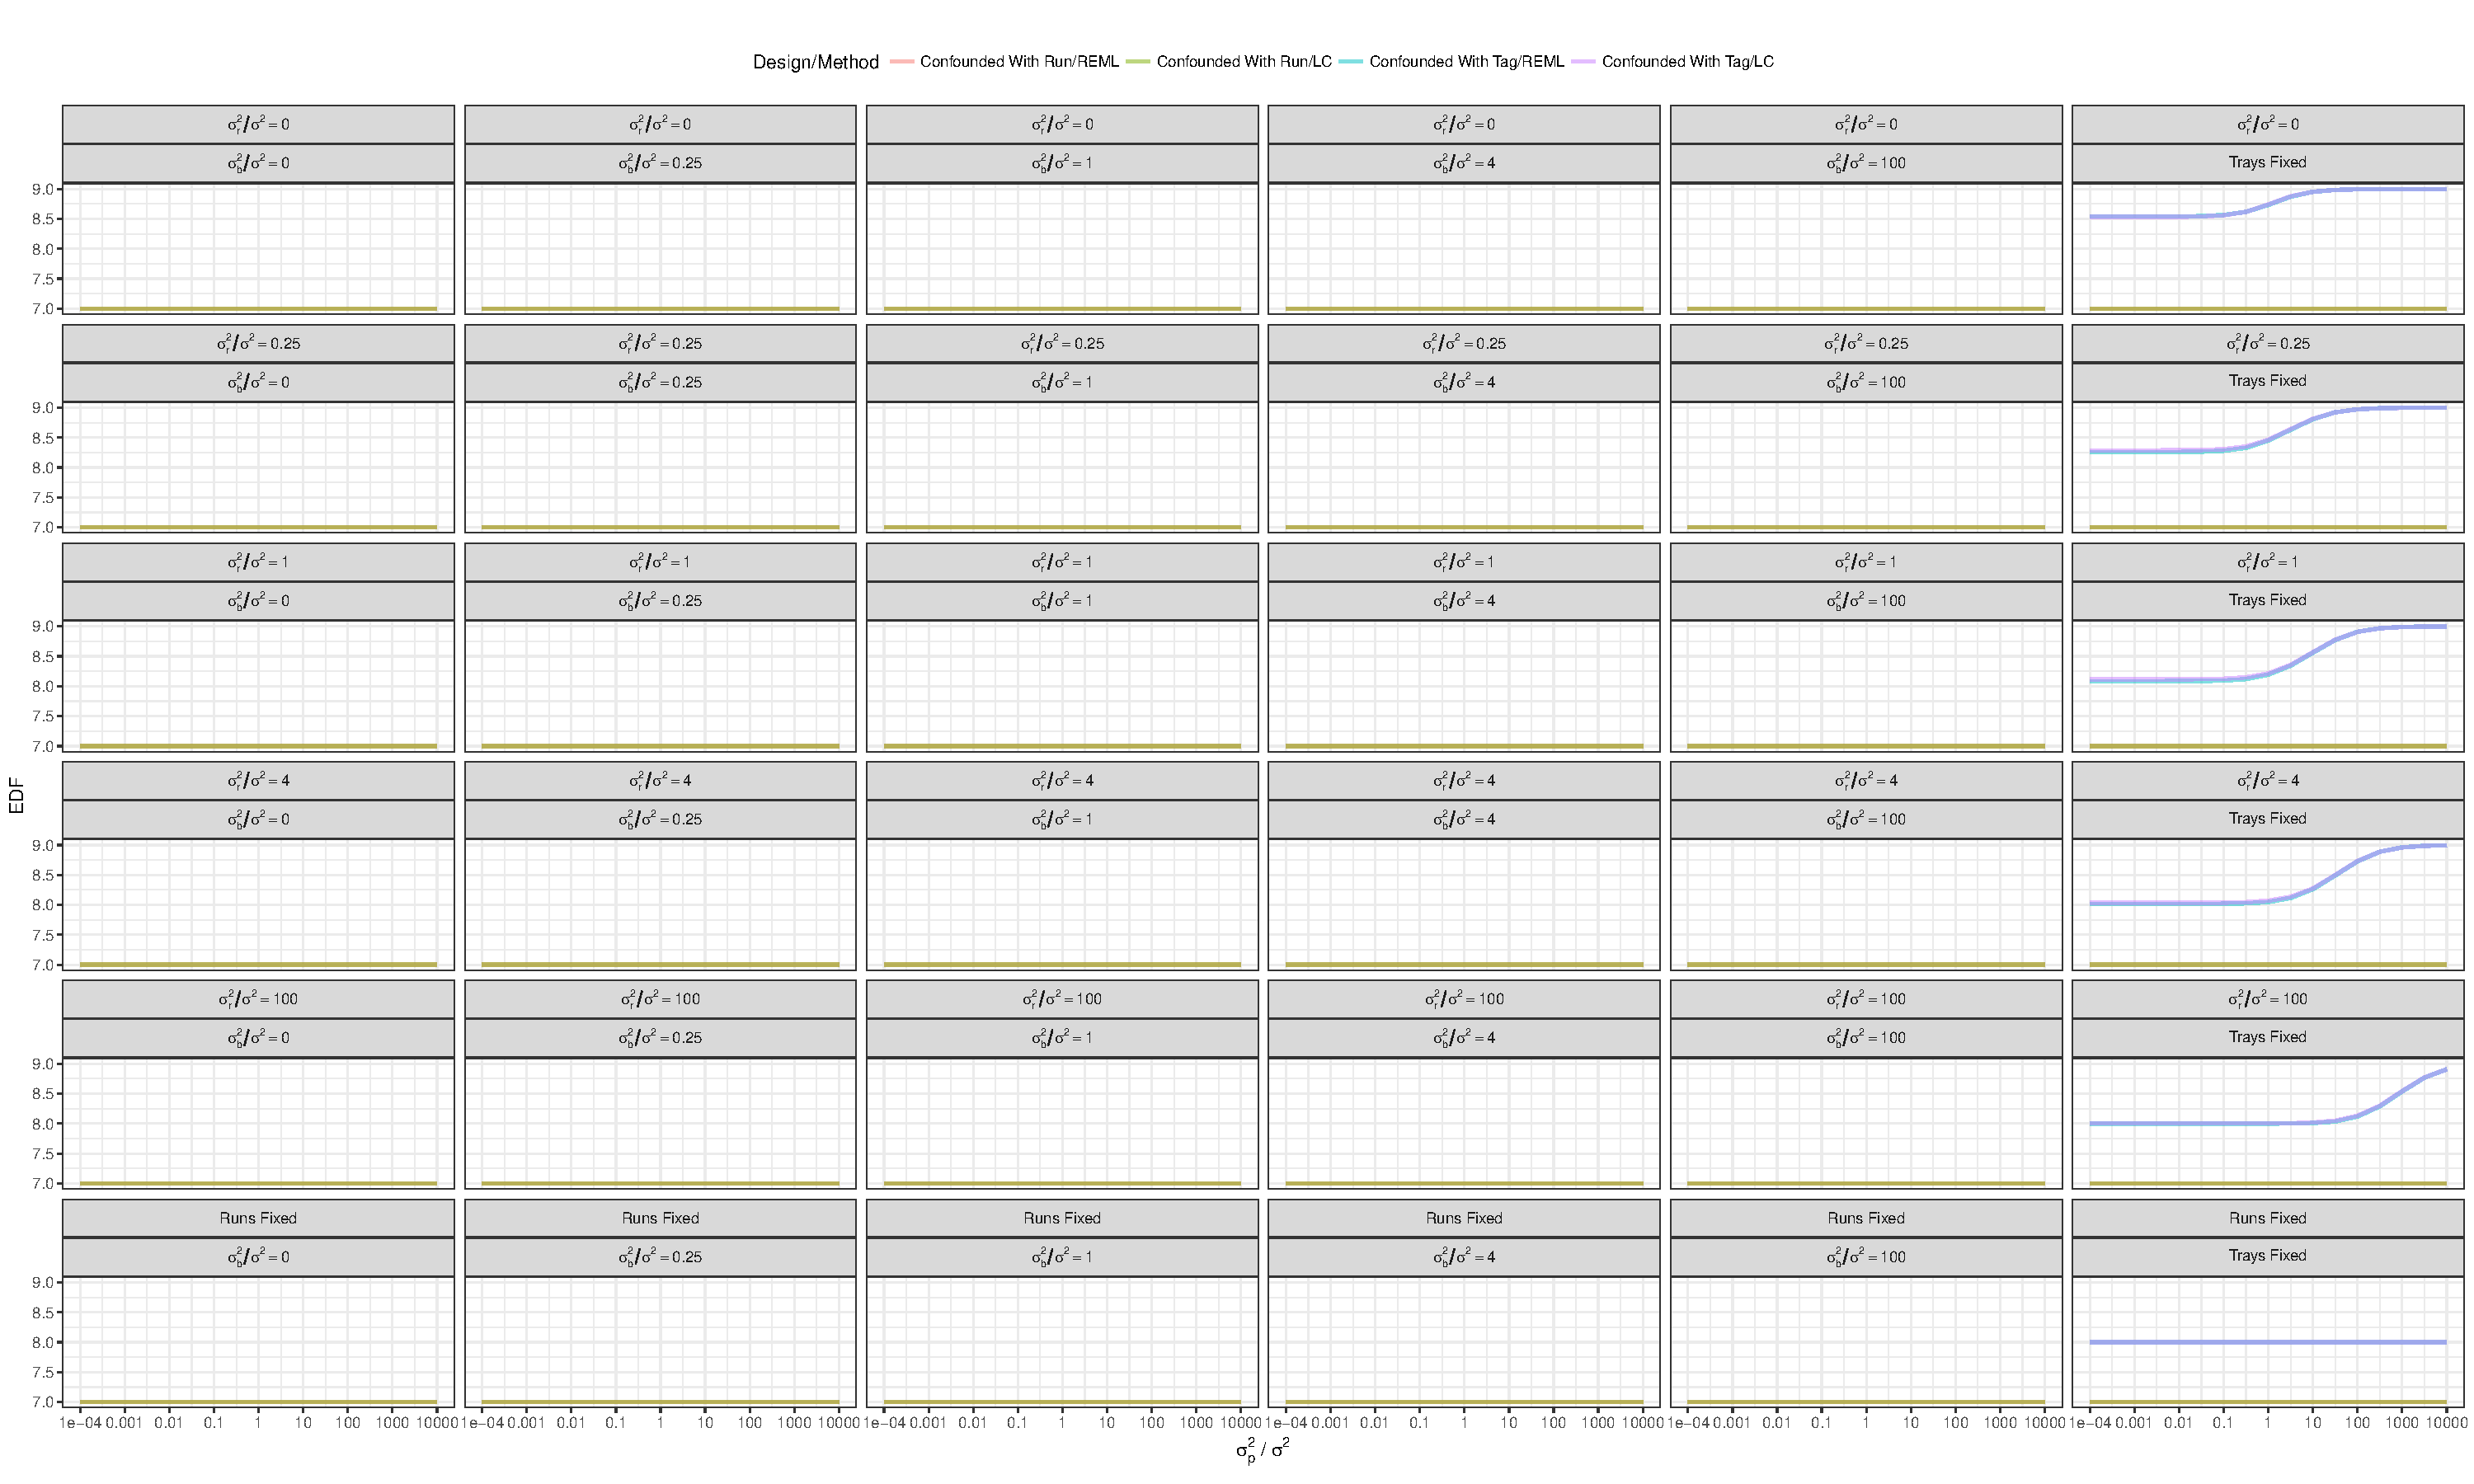
\includegraphics[width=1.3 \textwidth]{Chapter5/Graph/CRD44428.pdf}
\caption{EDF plots for optimal designs shown in Tables~\ref{tab:aniTrayDes3EDF} and \ref{tab:aniTrayDes4EDF}, where EDF is calculated using VCs estimated by both the REML and LC methods.}
\label{fig:RCBD442Tag8EDF}
\end{figure}
\end{landscape}

\subsection{Four-plex versus Eight-plex system}
From Figures~\ref{fig:RCBD442Tag4EDF} and ~\ref{fig:RCBD442Tag8EDF}, different ranges of values of the Between Tray VCs to measurement error ratio, denoted by $\sigma_{b}^2/\sigma^2$, did not change the EDF, because no extra information on the Between Plants VCs can be recovered from the Residual MS of the Between Tray Within Runs stratum and the Between Tray Within Runs stratum. Thus, Figure~\ref{fig:RCBD442Tag4vsTag8} only presents the EDF when Tray effects are assumed to be fixed, i.e.\ $\sigma_{b}^2 = \infty$, to make an overall comparison between the four- and eight-plex systems. 

Figure~\ref{fig:RCBD442Tag4vsTag8} shows the design when Tray effects are intentionally confounded with Tag effects with the eight-plex system being superior over the other three Phase 2 design options. However, there are three occasions when the EDF are the same between designs when Tray effects are intentionally confounded with Tag effects using the eight-plex system, and the design when Tray effects are intentionally confounded with Run effects using the four-plex system. The first occasion is when $\sigma_{r}^2/\sigma^2 = 4$ and $\sigma_{p}^2/\sigma^2$ is less than $0.1$, thus, run-to-run variation is 40 times that of plant-to-plant variation. The second occasion is when $\sigma_{r}^2/\sigma^2 = 100$ and  $\sigma_{p}^2/\sigma^2$ is less than 10, thus the run-to run variation is 10 times that of the plant-to-plant variation. The last occasion is when the Run effects are assumed to be fixed. Hence, the four-plex system will have the same precision as the eight-plex system when the run-to-run variation is 10 times higher than the plant-to-plant variation.  

\begin{figure}[h!]
\centering
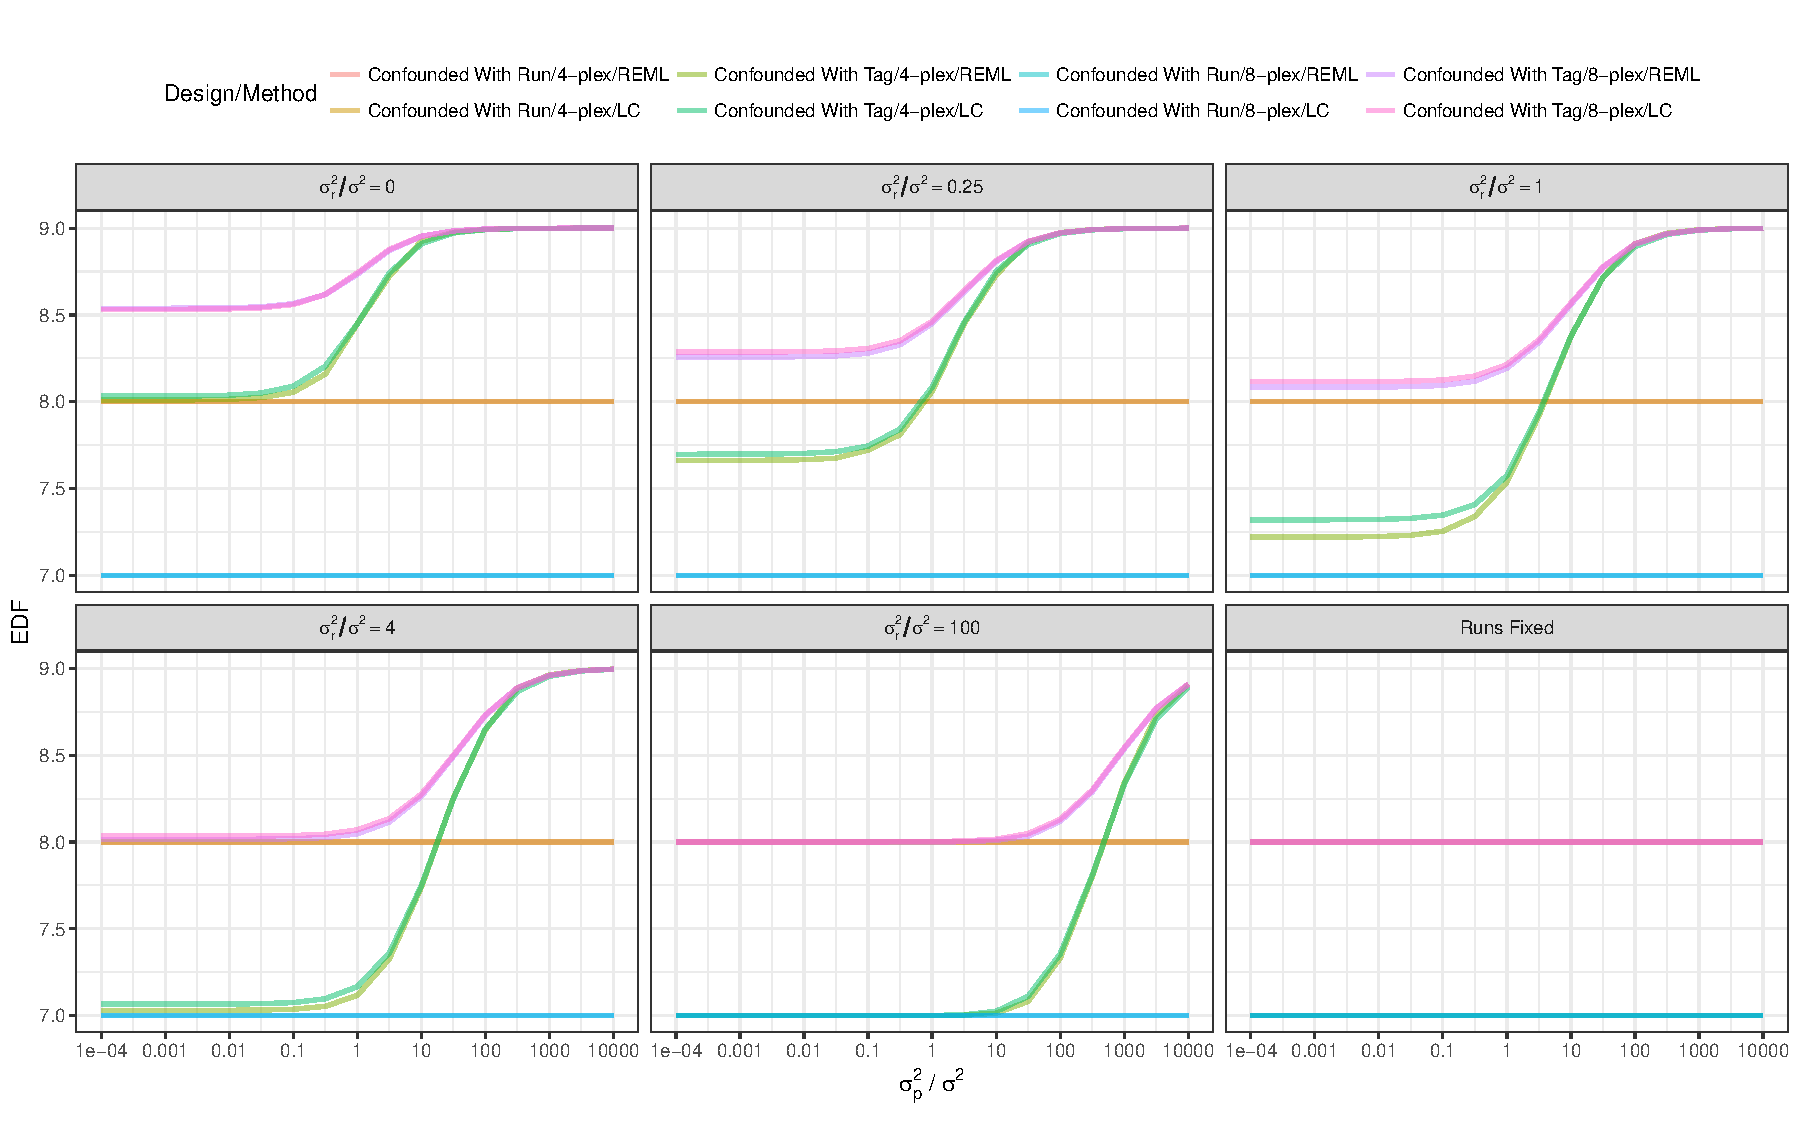
\includegraphics[width=1 \textwidth]{Chapter5/Graph/CRD44424vs8.pdf}
\caption{EDF for optimal designs shown in Tables~\ref{tab:aniTrayDes1EDF}, \ref{tab:aniTrayDes2EDF}, ~\ref{tab:aniTrayDes3EDF} and \ref{tab:aniTrayDes4EDF}, with Tray effects are assumed to be fixed, where EDF is calculated using VCs estimated by both the REML and LC methods.}
\label{fig:RCBD442Tag4vsTag8}
\end{figure}


\section{Summary}
\label{sec:conclusionChap5}
The Chapter described methods in estimating the VCs and approximating the EDF of Phase 2 experiments. EDF indicate how well we estimate the variances of Treatment effects, i.e. the Residual MS of the Between Experimental units stratum. Thus, the higher the EDF the better the estimates of the variance of Treatment effects and the valid F-test of the Treatment effects. We use EDF as another property with which to compare different optimal designs of the Phase 2 experiment found in Chapters 3 and 4. 

From all the EDF plots, we have shown that the REML method described here did not improve the approximation of the EDF from the optimal designs found in Chapters 3 and 4. This is due to these optimal designs having the property when the Phase 1 experimental units to the Phase 2 Blocks are always balanced, which ensures that we always have a valid F-test for testing for Treatment effects. Thus, these optimal designs are robust to the VC estimation procedure.

Three different cases were described when each case consists of the same Phase 1 design arranged in a CRD, comparing between using four-and eight-plex systems. The first case showed the four-plex system always generates higher EDF than the eight-plex system under different ranges of the VCs ratios. The second case showed when the EDF are always the same under different ranges of VCs ratios, because Treatment effects are completely confounded with Phase 2 Run effects, thus, the Run effects have to be assumed to be fixed. The last case showed an example when the four-plex system can have higher EDF than the eight-plex system, with run-to-run variation being higher than animal-to-animal variation, but the eight-plex system becomes better, with higher EDF, than the four-plex system when the animal-to-animal variation dominates.

The last part of the comparison was on the four different types of Phase 2 design with the same Phase 1 design arranged in a RCBD. These four different types of Phase 2 design comprised four-and eight-plex systems with two different confounding schemes when the Phase 1 Block (Tray) effects are intentionally confounded with the Phase 2 Tag and Run effects. We first showed that different ratios of Between Trays VCs to measurement error have no effects on the EDF. Further, the design when Phase 1 Block (Tray) effects are intentionally confounded with the Phase 2 Tag effects using the eight-plex system is preferable, as it generates the highest EDF among the four designs under all different combinations of the VCs. 


